\documentclass[11pt,a4paper]{article}

\usepackage[margin=2.5cm]{geometry}
\usepackage{amsmath,amssymb,amsthm,mathtools}
\usepackage{booktabs,tabularx,array}
\usepackage{enumitem}
\usepackage{microtype}
\usepackage{xcolor}
\usepackage{pgfplots}
\pgfplotsset{compat=1.18}
\usetikzlibrary{arrows.meta,positioning}
\usepackage{listings}
\usepackage[colorlinks=true,linkcolor=blue!50!black,citecolor=blue!50!black,urlcolor=blue!50!black]{hyperref}

\newcommand{\E}{\mathbb{E}}
\newcommand{\Var}{\mathrm{Var}}
\newcommand{\Wt}{\tilde W}
\newcommand{\AVF}{\mathrm{AVF}}
\newcommand{\LET}{\mathrm{LET}}
\newcommand{\dta}{\Delta t^{\alpha}}
\newcommand{\enc}{\mathrm{enc}}
\newcommand{\dec}{\mathrm{dec}}

\newtheorem{proposition}{Proposition}

\setlist{itemsep=2pt,topsep=4pt}

\lstset{
  language=C,
  basicstyle=\ttfamily\footnotesize,
  keywordstyle=\color{blue!50!black}\bfseries,
  commentstyle=\color{gray},
  columns=fullflexible,
  keepspaces=true,
  frame=single,
  rulecolor=\color{gray!40},
  xleftmargin=4pt,
  xrightmargin=4pt,
  breaklines=true,
  showstringspaces=false
}

\title{Single-Event Effects in Fractional-Order Reservoirs:\\ The Mathematics of Simulating Radiation Faults,\\ and a SPIRES Implementation Plan}
\author{Navid Shamszadeh}
\date{15 October 2026}

\begin{document}
\maketitle

\begin{abstract}
\noindent
Simulating radiation effects on digital hardware takes a chain of four models: the particle environment, the device's per-bit cross section, the architecture (which bits exist, how they encode values, how long a wrong value persists) and the application's own dynamics. This note derives the mathematics of each link. It applies them to a fractional-order spiking reservoir running the GL-FLIF model on fixed-point hardware, and ends with an implementation plan for SPIRES. The main results:
\begin{itemize}
  \item \textbf{The physics factors out.} The application-level failure rate is $\sum_c \lambda_c N_c\, \AVF_c$: per-bit upset rate, times bit count, times the probability that an upset in that storage class causes a failure. The device physics and the environment enter only through $\lambda_c$. Simulation therefore only has to estimate each $\AVF_c$ and the conditional error distribution, except where faults interact (multiple-cell upsets, high fluence, time-varying flux).
  \item \textbf{The number format decides what a bit flip means.} For every membrane potential in the operating range $[-65,-50]$~mV, 7 of the 64 possible flips of an IEEE-754 double multiply it by a factor between $2^{8}$ and $2^{512}$. In two's-complement fixed point the error is bounded by half the range, and a uniformly chosen flip produces a log-uniform error whose mean square comes 75\% from the top bit. Faults must be injected in the hardware's number format, not in the simulator's doubles.
  \item \textbf{The GL history buffer is the largest target, but it masks most of its own upsets.} An upset of size $\Delta$ in the sample that will next be read at lag $a$ injects a total forcing of exactly $\Delta(\varepsilon_{a-1} - \varepsilon_L)$. Summed over all slots this is $X_L = \alpha\,\Gamma(L+1-\alpha)/(\Gamma(2-\alpha)\Gamma(L)) \approx \alpha L^{1-\alpha}/\Gamma(2-\alpha)$. That is 31 at $\alpha = 0.5$, $L = 2999$, against 1 for an integer-order neuron. At equal particle fluence, configurations with different $\alpha$ and $L$ present different targets. They should therefore be compared at equal fluence, not at equal per-step fault probability.
  \item \textbf{The shared GL coefficients are a single point of failure.} Raising any $|c_k|$ by more than $\varepsilon_L + \dta/\tau_m$ makes the subthreshold dynamics of every neuron unstable. With UQ0.16 coefficients and the current Mackey--Glass configuration, an upset in any of the top 5 bits of any coefficient does this; the count is the top 3 bits at $\alpha = 0.3$ and the top 7 at $\alpha = 0.9$. Smaller upsets shift every neuron's operating point in proportion to the stored potential's distance from the representation's zero, so the voltage convention matters.
  \item \textbf{Most upsets map onto the existing dropout theory.} A spike-bit upset is the one-step transient fault of the dropout analysis. A refractory-counter upset is a transient dropout of log-uniformly distributed duration. A parameter upset repaired by scrubbing after $T_s$ leaves the same $t^{-1-\alpha}$ tail as a transient fault of duration $T_s$.
\end{itemize}
Notation follows the neuron-dropout analysis~\cite{dropout2026}, which this note extends.
\end{abstract}

\tableofcontents

%=====================================================================
\section{The modeling chain}
\label{sec:chain}

A radiation fault study answers one question: at a given particle environment, how often does the application fail, and how badly? Four models connect the particle to the failure (Figure~\ref{fig:chain}).

\begin{figure}[h]
\centering
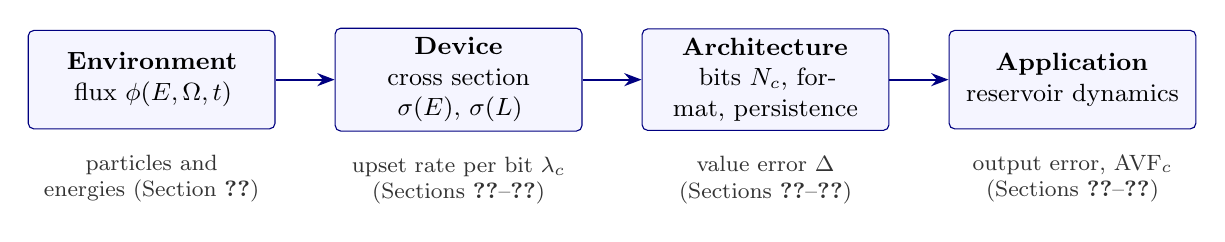
\begin{tikzpicture}[
  box/.style={draw=blue!50!black, rounded corners=2pt, align=center, font=\small, minimum height=1.25cm, text width=2.9cm, fill=blue!4},
  lab/.style={font=\footnotesize, align=center, text=gray!40!black},
  arr/.style={-{Stealth[length=2.2mm]}, thick, blue!50!black}
]
\node[box] (env) {\textbf{Environment}\\ flux $\phi(E,\Omega,t)$};
\node[box, right=0.75cm of env] (dev) {\textbf{Device}\\ cross section $\sigma(E)$, $\sigma(L)$};
\node[box, right=0.75cm of dev] (arch) {\textbf{Architecture}\\ bits $N_c$, format, persistence};
\node[box, right=0.75cm of arch] (app) {\textbf{Application}\\ reservoir dynamics};
\draw[arr] (env) -- (dev);
\draw[arr] (dev) -- (arch);
\draw[arr] (arch) -- (app);
\node[lab, below=0.2cm of dev] {upset rate per bit $\lambda_c$\\ (Sections~\ref{sec:physics}--\ref{sec:rates})};
\node[lab, below=0.2cm of arch] {value error $\Delta$\\ (Sections~\ref{sec:formats}--\ref{sec:inventory})};
\node[lab, below=0.2cm of app] {output error, $\AVF_c$\\ (Sections~\ref{sec:classes}--\ref{sec:metrics})};
\node[lab, below=0.2cm of env] {particles and\\ energies (Section~\ref{sec:physics})};
\end{tikzpicture}
\caption{The four models of a radiation fault simulation and what passes between them.}
\label{fig:chain}
\end{figure}

\begin{enumerate}
  \item \textbf{Environment.} The flux of particles, by species, energy, direction and time.
  \item \textbf{Device.} For each kind of storage cell, the probability that a particle of a given energy or linear energy transfer (LET) flips it, expressed as a cross section. Folding the cross section against the flux gives an upset rate per bit, $\lambda_c$, for each storage class $c$.
  \item \textbf{Architecture.} Which bits the design stores, in which number formats, and how long a wrong bit survives before it is overwritten, scrubbed or corrected. This turns a flipped bit into a value error $\Delta$ in a named variable.
  \item \textbf{Application.} How the reservoir's dynamics turn that value error into an output error.
\end{enumerate}
When upsets are rare compared with the time the system takes to recover from one, they act independently. The rate of application-level failures is then
\begin{equation}
\Lambda_{\mathrm{fail}} = \sum_{c} \lambda_c \, N_c \, \AVF_c,
\qquad
\AVF_c = \Pr\left(\text{failure} \mid \text{one upset in a random bit of class } c\right),
\label{eq:factor}
\end{equation}
where $N_c$ is the number of bits in class $c$ and $\AVF_c$ is its architectural vulnerability factor~\cite{mukherjee2003}. The physics (the first two models) enters only through $\lambda_c$, and the dynamics (the last two) only through $\AVF_c$. A simulation therefore does not need to model particles at all. It needs to inject single upsets into the right bits in the right format and measure $\AVF_c$, together with the distribution of error size, duration and recovery time conditional on the upset. The physics is folded in afterwards with Eq.~\eqref{eq:factor}.

The factorization breaks in three places, and those are where the simulation must model the event process itself:
\begin{itemize}
  \item \textbf{Multiple-cell upsets.} One particle can flip several physically adjacent bits. Their joint effect is not the sum of single-bit effects, and it defeats single-error-correcting codes (Section~\ref{sec:mcu}).
  \item \textbf{High fluence.} When a second upset arrives before the system has recovered from the first, the effects interact (Section~\ref{sec:accel}). Accelerated simulations, which inject far more upsets than the real environment would, are in this regime.
  \item \textbf{Time-varying flux.} In orbit, the rate changes along the orbit and jumps during solar particle events. Failures that depend on accumulation, such as uncorrectable errors between scrubs, then depend on the time profile of the flux, not just its mean.
\end{itemize}

\paragraph{Notation.} Storage classes are indexed by $c$, bits within a word by $k$ (with $k=0$ the least significant), and words by $w$. A word has $W$ bits, $F$ of them fractional. $\lambda$ denotes a rate per bit and $\Lambda$ a total rate. The reservoir notation is that of~\cite{dropout2026}: GL coefficients $c_k = (-1)^k\binom{\alpha}{k}$, buffer length $L$ (in SPIRES, $L = T_{\mathrm{mem}}/dt - 1$), truncation leak $\varepsilon_L$, membrane filter $\eta(z)$, DC gain $G_{\mathrm{DC}}$, linear reservoir matrix $A$ and fractional impulse response $G(t)$. The GL-FLIF update is
\begin{equation}
V_{i,n} = \dta\left( -\frac{V_{i,n-1} - V_{\mathrm{rest}}}{\tau_m} + I_{i,n} + b \right) - \sum_{k=1}^{L} c_k \, V_{i,n-k},
\qquad
I_{i,n} = \sum_j W_{ij}\, s_{j,n-1} + \sum_m W^{\mathrm{in}}_{im}\, u_{m,n},
\label{eq:glflif}
\end{equation}
with spike, reset to $V_{\mathrm{reset}}$ and refractory hold when $V_{i,n} \ge V_{\mathrm{th}}$.

The partial sums of the GL coefficients appear throughout:
\begin{equation}
\varepsilon_K = \sum_{k=0}^{K} c_k = (-1)^K\binom{\alpha-1}{K} = \frac{\Gamma(K+1-\alpha)}{\Gamma(1-\alpha)\,\Gamma(K+1)} \approx \frac{K^{-\alpha}}{\Gamma(1-\alpha)},
\qquad \varepsilon_0 = 1,
\label{eq:epsK}
\end{equation}
so $\sum_{k=1}^{K} |c_k| = 1 - \varepsilon_K$ for $0 < \alpha < 1$. The truncation leak of~\cite{dropout2026} is $\varepsilon_L$.

%=====================================================================
\section{Radiation effects and their digital abstractions}
\label{sec:taxonomy}

Radiation effects split into single-event effects, caused by one particle, and cumulative effects, caused by dose accumulated over time~\cite{petersen2011,dodd2003,baumann2005}. Table~\ref{tab:taxonomy} lists them with the fault model each becomes once lifted to the level of bits and variables.

\begin{table}[h]
\centering
\small
\begin{tabularx}{\textwidth}{@{}l>{\raggedright\arraybackslash}p{3.6cm}>{\raggedright\arraybackslash}p{2.4cm}>{\raggedright\arraybackslash}X@{}}
\toprule
Effect & Mechanism & Persistence & Digital abstraction and reservoir fault model \\
\midrule
SEU & Charge collected at a storage node exceeds its critical charge & Until overwritten, scrubbed or corrected & Bit flip in one stored word: neuron state, history, spike, counter, weight, coefficient \\
MCU / MBU & One particle upsets several adjacent cells & As SEU & Correlated flips in neighbouring bits; can defeat SEC-DED \\
SET & Transient pulse on a combinational net & One clock cycle, if latched & Wrong value written by one datapath operation, e.g.\ one corrupted GL update \\
SEFI & Upset in control logic or state machine & Until reset or power cycle & Freeze or reset of the whole reservoir \\
Configuration upset & Upset in SRAM FPGA configuration memory & Until scrubbed & Changed logic or routing: persistent functional fault, e.g.\ a stuck neuron unit \\
SEL & Parasitic thyristor turned on & Until power cycle; may be destructive & Total outage, then state loss; permanent dropout if damaged \\
SEB, SEGR & Burnout, gate rupture (power devices) & Permanent & Hard failure; out of scope \\
TID, DD & Trapped charge, lattice damage & Cumulative & Slow drift of timing and leakage; delay faults late in life; out of scope \\
\bottomrule
\end{tabularx}
\caption{Radiation effects and their fault models. SEU: single-event upset. MCU/MBU: multiple-cell or multiple-bit upset. SET: single-event transient. SEFI: single-event functional interrupt. SEL: single-event latch-up. TID: total ionizing dose. DD: displacement damage.}
\label{tab:taxonomy}
\end{table}

Two properties of this taxonomy shape the simulation.
\begin{itemize}
  \item \textbf{Persistence classes.} An upset in a \emph{dynamic} variable (membrane potential, history, spikes, counters) is overwritten by the computation itself, so it is transient by construction. An upset in a \emph{parameter} (weights, coefficients, gains, configuration) persists until something repairs it. The two classes act on the reservoir as additive and multiplicative faults in the sense of~\cite{blanke2016}, and they have different recovery dynamics (Section~\ref{sec:response}).
  \item \textbf{Scope.} An upset in a per-neuron variable perturbs one neuron. An upset in a shared resource (the coefficient memory, the buffer pointer, the input gain, a time-multiplexed update unit) perturbs every neuron at once. Shared resources are few bits but common-mode, and they dominate the catastrophic outcomes (Section~\ref{sec:coeff}).
\end{itemize}
Neuron dropout, the fault studied so far~\cite{dropout2026}, is the abstraction of a permanent failure (SEL damage, a configuration upset in a neuron's update logic held until scrub) or of a transient one (a refractory-counter upset, Section~\ref{sec:refrac}). It is one class among several, with its own physical rate.

%=====================================================================
\section{From particle to upset}
\label{sec:physics}

\subsection{Environments}

\begin{itemize}
  \item \textbf{Terrestrial.} Cosmic rays striking the atmosphere produce a cascade whose ground-level component that matters most is neutrons. Fast neutrons ($E > 10$~MeV) upset cells through nuclear reactions in silicon that produce short-range, highly ionizing recoils. The JEDEC reference flux for New York City at sea level is about $13~\mathrm{cm^{-2}\,h^{-1}}$ above 10~MeV~\cite{jesd89a,gordon2004}; it scales with altitude (roughly a factor of 300 at aircraft altitude) and geomagnetic latitude~\cite{normand1996}. Thermal neutrons upset cells through $^{10}$B capture in borophosphosilicate glass, and alpha particles come from trace radioactivity in packaging and solder~\cite{may1979,baumann2005}.
  \item \textbf{Space.} Three populations: galactic cosmic rays (protons through iron-group nuclei with energies up to GeV per nucleon, which upset cells by direct ionization), protons trapped in the radiation belts (including the South Atlantic Anomaly in low Earth orbit) and solar particle events, which raise the flux by orders of magnitude for hours to days. Environment models such as CREME96~\cite{tylka1997} turn an orbit and shielding thickness into differential spectra $\phi(E)$ for protons and LET spectra $\phi(L)$ for heavy ions.
\end{itemize}

\subsection{Energy deposition}

A charged particle loses energy along its path at a rate set by its stopping power. Normalized by the material's density this is the linear energy transfer, $\LET = (1/\rho)\, dE/dx$, quoted in $\mathrm{MeV\,cm^2\,mg^{-1}}$. Each electron--hole pair in silicon costs $E_{eh} \approx 3.6$~eV, so the charge freed along a path of length $\ell$ is
\begin{equation}
Q_{\mathrm{dep}} = \frac{q\,\rho}{E_{eh}} \int_0^{\ell} \LET(x)\,dx \;\approx\; \frac{q\,\rho\,\LET\,\ell}{E_{eh}},
\qquad
\frac{q\rho}{E_{eh}} \approx 10.4~\mathrm{fC\,\mu m^{-1}} \text{ per } \mathrm{MeV\,cm^2\,mg^{-1}},
\label{eq:qdep}
\end{equation}
with $\rho = 2330~\mathrm{mg\,cm^{-3}}$ for silicon. The approximation holds when LET is roughly constant over the sensitive depth, which is true for heavy ions crossing a thin sensitive volume. A particle with $\LET = 1~\mathrm{MeV\,cm^2\,mg^{-1}}$ crossing 1~$\mu$m of silicon frees about 10~fC. Critical charges of deep-submicron SRAM cells are of the order of 1~fC~\cite{baumann2005}, so even light ions upset modern memories. Protons and neutrons rarely deposit enough by direct ionization. They act indirectly: a nuclear reaction produces a recoil nucleus, and the recoil's LET does the damage. Their cross sections are therefore parametrized by the incident particle's energy, not by its LET (Section~\ref{sec:sigma}).

\subsection{Charge collection and the current pulse}

Only charge collected at a sensitive junction matters. Collection has a prompt drift component (including funneling of the junction field along the ion track) and a slower diffusion component~\cite{dodd2003}. Circuit simulations represent the collected charge $Q_{\mathrm{coll}}$ as a current source at the struck node, usually the double exponential of Messenger~\cite{messenger1982}:
\begin{equation}
I(t) = \frac{Q_{\mathrm{coll}}}{\tau_{a} - \tau_{b}} \left( e^{-t/\tau_{a}} - e^{-t/\tau_{b}} \right), \qquad \tau_a > \tau_b,
\label{eq:dexp}
\end{equation}
where $\tau_a$ is the collection time constant and $\tau_b$ the time to establish the track. The pulse integrates to $Q_{\mathrm{coll}}$. Typical constants are tens to hundreds of picoseconds.

\subsection{The upset criterion}

A storage cell is a bistable circuit. The pulse of Eq.~\eqref{eq:dexp} pulls the struck node toward the opposite rail while the cell's feedback restores it. The cell flips if the collected charge exceeds a critical charge:
\begin{equation}
\text{upset} \iff Q_{\mathrm{coll}} > Q_{\mathrm{crit}}, \qquad Q_{\mathrm{crit}} \approx C_{\mathrm{node}}\, V_{DD} + I_{\mathrm{restore}}\, t_{\mathrm{flip}}.
\label{eq:qcrit}
\end{equation}
The first term is the charge needed to swing the node capacitance; the second is the charge the restoring transistor supplies during the cell's flip time. Because both terms shrink with feature size and supply voltage, the per-bit upset rate does too, though more slowly than density grows. Hazucha and Svensson~\cite{hazucha2000} fit the terrestrial neutron rate per cell with
\begin{equation}
\mathrm{SER} = K\, F\, A_{\mathrm{diff}}\, \exp\left( -Q_{\mathrm{crit}}/Q_s \right),
\label{eq:hazucha}
\end{equation}
where $F$ is the neutron flux above 10~MeV, $A_{\mathrm{diff}}$ the sensitive drain area, $Q_s$ a charge-collection efficiency that also shrinks with scaling, and $K$ a technology constant. The exponential is why hardening by raising $Q_{\mathrm{crit}}$ (larger nodes, added capacitance, dual-interlocked cells) is effective.

Charge spreading from one track to neighbouring nodes produces multiple-cell upsets. Their share grows with LET, incidence angle and integration density~\cite{reed1997,quinn2005}.

\subsection{Transients in combinational logic}

A strike on a combinational node produces a voltage pulse of width $w$ that propagates toward the registers. It corrupts state only if it survives three kinds of masking~\cite{shivakumar2002}:
\begin{itemize}
  \item \textbf{Logical masking.} A gate whose output does not depend on the struck input at that moment blocks the pulse (an AND gate with another input at 0).
  \item \textbf{Electrical masking.} Each gate attenuates the pulse; pulses narrower than about one gate delay die out.
  \item \textbf{Latching-window masking.} A register captures the wrong value only if the pulse covers its setup-and-hold window $t_w$ at a clock edge. For a pulse arriving at a uniformly random time,
  \begin{equation}
  P_{\mathrm{latch}}(w) = \min\!\left(1,\ \max\!\left(0,\ \frac{w - t_w}{T_{\mathrm{clk}}}\right)\right).
  \label{eq:platch}
  \end{equation}
\end{itemize}
The transient error rate of a block is $\sum_{\mathrm{nodes}} R_{\mathrm{node}}\, P_{\mathrm{logical}}\, P_{\mathrm{electrical}}\, P_{\mathrm{latch}}$. Because $P_{\mathrm{latch}} \propto 1/T_{\mathrm{clk}}$, transient errors grow linearly with clock frequency, while storage upsets do not depend on it. At the architectural level, a latched transient is an upset in the register that latched it, occurring at a clock edge. For the reservoir that means a corrupted result of one GL update (Section~\ref{sec:set}).

\subsection{Why a bit flip is the right abstraction}

Once the cell has flipped, its feedback holds the new value: the analog event has left behind a valid but wrong digital state. For storage cells the bit-flip model is therefore exact at the architectural level. The only physics that survives into the digital model is \emph{which} bits flip together (multiple-cell upsets) and \emph{when} (the arrival process). For transients the bit-flip model is an approximation: it summarizes the masking factors in one probability and places the error at a clock edge. For configuration upsets in SRAM FPGAs it is exact at the bit level but not at the functional level, because the effect of a configuration bit depends on the placed-and-routed netlist (Section~\ref{sec:config}).

%=====================================================================
\section{Cross sections and upset rates}
\label{sec:rates}

\subsection{Cross sections}
\label{sec:sigma}

A beam test exposes a device to a fluence $\Phi$ (particles per cm$^2$) and counts upsets. The per-bit cross section is
\begin{equation}
\sigma = \frac{N_{\mathrm{upsets}}}{\Phi\, N_{\mathrm{bits}}} \quad [\mathrm{cm^2\,bit^{-1}}],
\end{equation}
the effective area per bit that a particle must hit to cause an upset. It is measured as a function of LET for heavy ions and of energy for protons and neutrons, and is fitted with standard forms.
\begin{itemize}
  \item \textbf{Heavy ions: the Weibull fit.}
  \begin{equation}
  \sigma(L) = \sigma_{\mathrm{sat}} \left\{ 1 - \exp\left[ -\left( \frac{L - L_0}{W_L} \right)^{s} \right] \right\} \quad (L > L_0), \qquad \sigma(L) = 0 \quad (L \le L_0),
  \label{eq:weibull}
  \end{equation}
  with saturation cross section $\sigma_{\mathrm{sat}}$, threshold LET $L_0$, width $W_L$ and shape $s$~\cite{petersen2011}.
  \item \textbf{Protons: the two-parameter Bendel fit}~\cite{stapor1990,bendel1983}.
  \begin{equation}
  \sigma(E) = \left( \frac{B}{A} \right)^{14} \left[ 1 - \exp\left( -0.18\, Y^{1/2} \right) \right]^{4} \times 10^{-12}~\mathrm{cm^2\,bit^{-1}}, \qquad Y = \left( \frac{18}{A} \right)^{1/2} (E - A),
  \label{eq:bendel}
  \end{equation}
  for $E > A$ (in MeV) and zero below. $A$ acts as a threshold energy; $B$ sets the saturation level. The one-parameter form of Bendel and Petersen fixes $B = 24$. A Weibull in energy is also common.
  \item \textbf{Neutrons.} Usually a single cross section measured in a spallation beam whose spectrum resembles the atmospheric one, so that the terrestrial rate is $\sigma_n \times$ (reference flux) directly~\cite{jesd89a}.
\end{itemize}
Cross sections can differ between the $0\to1$ and $1\to0$ directions, so the rate of a bit can depend on its value. The simulation can carry this as a per-direction weight (Section~\ref{sec:impl}).

\subsection{Rate integrals}

For an isotropic environment of protons or neutrons with differential flux $\phi(E)$, the per-bit rate is the fold
\begin{equation}
\lambda = \int \sigma(E)\, \phi(E)\, dE.
\label{eq:rate_e}
\end{equation}
For heavy ions the cross section depends on the charge deposited in the sensitive volume, which depends on path length and so on direction. The rectangular parallelepiped (RPP) model~\cite{pickel1978,petersen2011} treats the sensitive volume as a box with surface area $S$. For a convex body in an isotropic field, particles of omnidirectional flux $F$ hit it at the rate $FS/4$, and their chord lengths $p$ follow a geometric distribution $D(p)$. An upset needs $\rho\, \LET\, p \ge E_c$, where $E_c = Q_{\mathrm{crit}} E_{eh}/q$ is the critical energy, so
\begin{equation}
\lambda_{\mathrm{RPP}} = \frac{S}{4} \int_{p_{\min}}^{p_{\max}} F\!\left( \frac{E_c}{\rho\, p} \right) D(p)\, dp,
\label{eq:rpp}
\end{equation}
where $F(L)$ is the integral omnidirectional flux of particles with LET above $L$. Real devices do not have one sharp threshold. The integral RPP (IRPP) method used by CREME96~\cite{tylka1997} averages Eq.~\eqref{eq:rpp} over a distribution of critical LETs given by the normalized Weibull curve, $\lambda_{\mathrm{IRPP}} = \int \lambda_{\mathrm{RPP}}(L_c)\, \sigma_{\mathrm{sat}}^{-1}\, (d\sigma/dL)(L_c)\, dL_c$. For a quick estimate, Petersen's figure of merit~\cite{petersen1983fom} gives $\lambda \approx C\, \sigma_{\mathrm{sat}} / L_{0.25}^{2}$, where $L_{0.25}$ is the LET at which $\sigma = \sigma_{\mathrm{sat}}/4$ and $C$ is an orbit-dependent constant tabulated in~\cite{petersen2011}.

Upset rates are quoted as upsets per bit per day (space) or in FIT, failures per $10^9$ device-hours, usually per megabit (terrestrial). The conversion is
\begin{equation}
\lambda\,[\mathrm{bit^{-1}\,s^{-1}}] = \frac{\mathrm{FIT/Mbit}}{3600 \times 10^{9} \times 10^{6}}.
\end{equation}

\subsection{From physical time to simulation steps}
\label{sec:timebase}

The reservoir advances in micro-steps. On hardware each micro-step takes $\tau_{\mathrm{step}} = n_{\mathrm{cyc}}/f_{\mathrm{clk}}$ seconds, with $n_{\mathrm{cyc}}$ clock cycles per micro-step. The expected number of upsets in class $c$ per micro-step is
\begin{equation}
\mu_c = K \, \lambda_c \, N_c \, \tau_{\mathrm{step}},
\label{eq:mu}
\end{equation}
where $K \ge 1$ is an acceleration factor. With $K=1$ upsets are vanishingly rare. For illustration take $\lambda = 10^{-16}~\mathrm{bit^{-1}\,s^{-1}}$ (360~FIT/Mbit, a typical order of magnitude for unhardened terrestrial SRAM~\cite{baumann2005}) and the 20.5~Mbit design of Section~\ref{sec:inventory}. The reservoir then sees one upset every 15 years. The existing Mackey--Glass experiment injects a fault with probability 0.05 per macro-step, which for any plausible $\tau_{\mathrm{step}}$ corresponds to an acceleration factor above $10^{10}$. Acceleration is legitimate only within the limit of Section~\ref{sec:accel}.

%=====================================================================
\section{The arrival process}
\label{sec:arrivals}

\subsection{Poisson arrivals}

Particle arrivals are independent, so upsets in a bit form a Poisson process. Superposing independent Poisson processes gives a Poisson process, so the whole design sees upsets at total rate $\Lambda = \sum_c \lambda_c N_c$. Conversely, each upset belongs to class $c$ with probability
\begin{equation}
\pi_c = \frac{\lambda_c N_c}{\Lambda},
\label{eq:pic}
\end{equation}
independently of the others (thinning), and within a class to a uniformly chosen bit, or to a bit chosen in proportion to its own cross section if bits differ. Three equivalent ways to generate the process in simulation:
\begin{itemize}
  \item \textbf{Counts per step.} The number of upsets in a micro-step is Poisson with mean $\mu = \sum_c \mu_c$.
  \item \textbf{Inter-arrival times.} The gaps between upsets are independent exponentials with mean $1/\mu$ steps. Drawing the next arrival time in advance costs nothing per step, which matters when $\mu \ll 1$.
  \item \textbf{Fixed count.} Conditional on $n$ upsets in a window, their times are independent and uniform over it. This is the basis of the single-upset campaign (Section~\ref{sec:metrics}).
\end{itemize}
The time to the first upset is exponential, so the reliability with respect to upsets of class $c$ alone is $R_c(t) = \exp(-\lambda_c N_c t)$.

\paragraph{The Bernoulli approximation.} Firing a fault with probability $p$ per step, as the existing experiment does, approximates a Poisson process of mean $\mu = -\ln(1-p) \approx p$ per step but never places two upsets in one step. That is harmless for small $p$. The real problem is elsewhere. A fixed $p$ per step does not scale with the number of bits, so it makes a large design look exactly as exposed as a small one. Section~\ref{sec:fluence} shows why that matters for comparisons across $\alpha$ and $L$.

\subsection{Time-varying flux}

In orbit, $\lambda_c(t)$ varies along the orbit and with solar activity. A non-homogeneous Poisson process is generated by thinning~\cite{lewis1979}: draw candidate arrivals at a constant rate $\bar\mu \ge \max_t \mu(t)$ and keep each candidate at time $t$ with probability $\mu(t)/\bar\mu$. The number of upsets in an interval is then Poisson with mean $\int \mu(t)\,dt$.

\subsection{Multiple-cell upsets}
\label{sec:mcu}

A particle event can flip a cluster of $M \ge 1$ adjacent cells. Events form a Poisson process at rate $\Lambda_e$, and the bit-upset rate is $\Lambda_e \E[M]$, a compound Poisson process. In the absence of measured cluster-size data, a geometric size distribution is a reasonable parametric form,
\begin{equation}
\Pr(M = m) = (1-\theta)\, \theta^{m-1}, \qquad \E[M] = \frac{1}{1-\theta},
\end{equation}
with $\theta$ fitted to the measured MCU fraction $\Pr(M \ge 2) = \theta$. Clusters are contiguous in the \emph{physical} array, so their logical effect depends on the layout. With column interleaving of factor $I$, physically adjacent cells belong to $I$ different words, and a cluster of size $M \le I$ flips at most one bit per word. Without interleaving the same cluster flips $M$ adjacent bits of one word. Since the physical layout is rarely known in simulation, $\theta$ and $I$ should be swept parameters.

\subsection{Accumulation, error correction and scrubbing}
\label{sec:ecc}

Parameters persist until repaired, so their upsets accumulate. Three repair mechanisms matter.
\begin{itemize}
  \item \textbf{Scrubbing without error correction} (for example rewriting the configuration memory, or reloading weights from a protected copy) clears every error at period $T_s$. A persistent upset then lasts until the next scrub. For uniformly arriving upsets the mean exposure is $T_s/2$.
  \item \textbf{SEC-DED with scrubbing}~\cite{hsiao1970,saleh1990}. A word of $n$ bits (including check bits) survives any single upset. It fails if two of its bits are upset within one scrub interval. The number of upsets in a word during an interval is Poisson with mean $\nu = n\lambda T_s$, so
  \begin{equation}
  \Pr(\text{uncorrectable}) = 1 - e^{-\nu}(1+\nu) \approx \frac{\nu^2}{2},
  \qquad
  \Lambda_{\mathrm{unc}} \approx \frac{M_w\, n^2 \lambda^2 T_s}{2}
  \label{eq:secded}
  \end{equation}
  for $M_w$ words. The rate falls linearly with the scrub period and quadratically with the per-bit rate. Multiple-cell upsets add $\Lambda_e \Pr(\text{a cluster hits two bits of one word})$, which interleaving drives to zero for clusters up to size $I$.
  \item \textbf{Triple modular redundancy with voting}~\cite{lyons1962}. Without repair the reliability is $R_{\mathrm{TMR}} = 3R^2 - 2R^3$, better than $R$ only while $R > 1/2$. With bitwise voting every $T_v$ (for state, every update), a word fails only if two replicas are upset in the same bit within one voting interval, at rate about $3 n \lambda^2 T_v$ per word.
\end{itemize}

\subsection{When acceleration is valid}
\label{sec:accel}

Accelerated simulation multiplies all rates by $K$. Its results transfer to the real environment only when the extra upsets do not interact, that is, when a second upset rarely arrives while the system is still recovering from the first. If $T_{\mathrm{rec}}$ is the recovery time (Section~\ref{sec:response}), the probability that an upset overlaps another is
\begin{equation}
P_{\mathrm{overlap}} = 1 - \exp\left( -K \Lambda\, T_{\mathrm{rec}} \right) \approx K \Lambda T_{\mathrm{rec}},
\label{eq:overlap}
\end{equation}
and acceleration is valid while $K \Lambda T_{\mathrm{rec}} \ll 1$. Fractional reservoirs need particular care because their recovery is slow: with the buffer cap of~\cite{dropout2026}, $T_{\mathrm{rec}}$ is up to a few $L$ micro-steps. In the existing experiment, $p = 0.05$ per macro-step and $L\,dt = 300$ macro-steps give $K \Lambda T_{\mathrm{rec}} \approx 15$: every fault overlaps many others, so it measures the cumulative regime, not single-upset vulnerability. Both regimes are worth measuring, but separately (Section~\ref{sec:metrics}).

%=====================================================================
\section{From bit flip to value error: number formats}
\label{sec:formats}

The same physical event produces errors of entirely different size and character depending on how the hardware encodes the value. This is the single most important modeling decision in the simulation.

\subsection{Two's-complement fixed point}

A $W$-bit word with $F$ fractional bits represents
\begin{equation}
x = 2^{-F}\left( -b_{W-1}\, 2^{W-1} + \sum_{k=0}^{W-2} b_k\, 2^{k} \right) \in \left[ -2^{W-1-F},\ 2^{W-1-F} \right).
\end{equation}
Flipping bit $k$ changes the value by exactly
\begin{equation}
\Delta x = (1 - 2 b_k)\, 2^{k-F} \quad (k < W-1), \qquad \Delta x = (2 b_{W-1} - 1)\, 2^{W-1-F} \quad (\text{sign bit}).
\label{eq:fixflip}
\end{equation}
The sign of the error depends on the stored bit, but its magnitude does not depend on the value.

\begin{proposition}[Fixed-point flip errors are log-uniform]
\label{prop:loguniform}
If the flipped bit is uniform on $\{0,\dots,W-1\}$, then $\log_2|\Delta x|$ is uniform on $\{-F, \dots, W-1-F\}$. The mean square error is
\begin{equation}
\E[\Delta x^2] = \frac{4^{-F}}{W} \cdot \frac{4^{W}-1}{3},
\end{equation}
and the top $j$ bits contribute the fraction $(4^{W} - 4^{W-j})/(4^{W}-1) \approx 1 - 4^{-j}$ of it.
\end{proposition}
\begin{proof}
By Eq.~\eqref{eq:fixflip}, $|\Delta x| = 2^{k-F}$ for bit $k$, including the sign bit. Summing $4^{k-F}$ over $k$ gives the geometric series.
\end{proof}
The top bit alone carries 75\% of the mean square error and the top two carry 94\%. Error magnitudes span the full dynamic range of the format with equal probability per octave. Two consequences follow. Most upsets are small and are masked by the dynamics, while a few are as large as the format allows. And protecting only the top few bits of each word (by parity, duplication or range checks) removes almost all of the mean square error at a fraction of the cost of protecting the whole word (Section~\ref{sec:mitigation}).

Unsigned formats such as the UQ0.16 coefficients of~\cite{mastin2026} have $\Delta x = (1-2b_k)2^{k-F}$ for every bit and range $[0, 2^{W-F})$. For a value much smaller than full scale, the high bits are all zero, so every high-bit flip is $0 \to 1$ and increases the value. For the GL coefficients this asymmetry decides the failure mode (Section~\ref{sec:coeff}).

\subsection{IEEE-754 floating point}

A binary64 value is $x = (-1)^{s}\, 2^{e-1023}\,(1 + f\,2^{-52})$ with an 11-bit exponent $e$ and 52-bit fraction $f$. A flip of
\begin{itemize}
  \item \textbf{fraction bit $k$} ($0 \le k \le 51$) changes $x$ by $\pm 2^{e-1023-52+k}$, a relative error between $2^{k-53}$ and $2^{k-52}$;
  \item \textbf{exponent bit $j$} ($0 \le j \le 10$, stored bit $52+j$) multiplies $x$ by $2^{\pm 2^{j}}$, or produces a subnormal, an infinity or a NaN when $e$ reaches 0 or 2047;
  \item \textbf{the sign bit} gives $x \to -x$.
\end{itemize}
Figure~\ref{fig:bitpos} shows the effect on a resting membrane potential. For every potential in the operating range $[-65,-50]$~mV the exponent is 1028 or 1029, so exponent bits 3--9 (stored bits 55--61) are 0 and their flips multiply $V$ by $2^{8}, 2^{16}, \dots, 2^{512}$. Bit 62 sends $V$ to about $10^{-307}$, effectively 0~mV, and the sign bit sends it to $+65$~mV; both put the potential far above threshold. Of the 64 flips, 14 change $V$ by more than the 15~mV gap between reset and threshold, and 7 make $|V| > 10^{4}$~mV. For values in $(-2,2)$, such as weights, coefficients and gains, the top exponent bit is 0 and its flip gives about $10^{307}$ or an infinity, so the next multiply-accumulate overflows. A NaN, once produced, propagates through every dot product it enters, including the readout.

\begin{figure}[h]
\centering
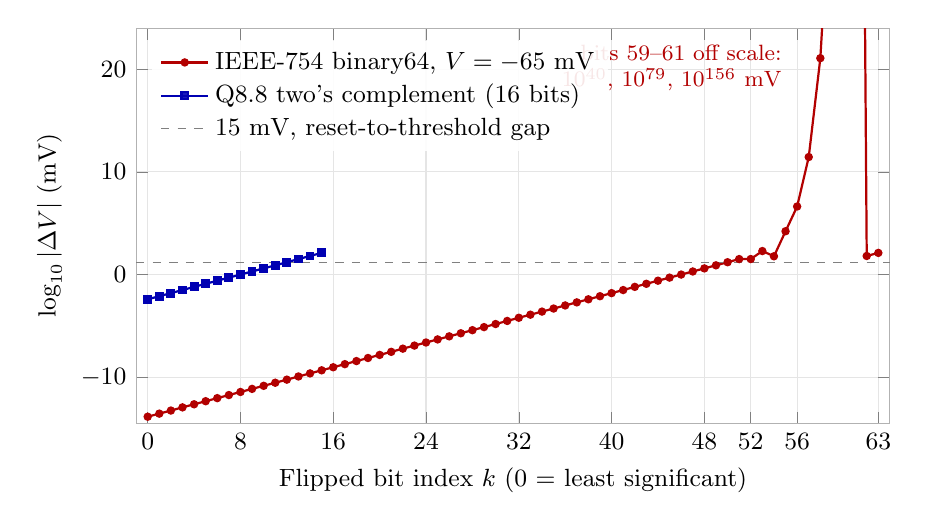
\begin{tikzpicture}
\begin{axis}[
  width=0.92\textwidth, height=6.6cm,
  xmin=-1, xmax=64, ymin=-14.5, ymax=24,
  xlabel={Flipped bit index $k$ (0 = least significant)},
  ylabel={$\log_{10}|\Delta V|$ (mV)},
  xtick={0,8,16,24,32,40,48,52,56,63},
  grid=major, grid style={gray!20},
  axis line style={gray!60},
  tick label style={font=\small},
  label style={font=\small},
  legend style={font=\small, draw=none, fill=white, fill opacity=0.9, text opacity=1, at={(0.02,0.97)}, anchor=north west},
  legend cell align=left,
  clip=true,
]
\addplot[color=red!70!black, thick, mark=*, mark size=1.1pt] coordinates {(0,-13.85) (1,-13.55) (2,-13.25) (3,-12.94) (4,-12.64) (5,-12.34) (6,-12.04) (7,-11.74) (8,-11.44) (9,-11.14) (10,-10.84) (11,-10.54) (12,-10.24) (13,-9.93) (14,-9.63) (15,-9.33) (16,-9.03) (17,-8.73) (18,-8.43) (19,-8.13) (20,-7.83) (21,-7.53) (22,-7.22) (23,-6.92) (24,-6.62) (25,-6.32) (26,-6.02) (27,-5.72) (28,-5.42) (29,-5.12) (30,-4.82) (31,-4.52) (32,-4.21) (33,-3.91) (34,-3.61) (35,-3.31) (36,-3.01) (37,-2.71) (38,-2.41) (39,-2.11) (40,-1.81) (41,-1.51) (42,-1.20) (43,-0.90) (44,-0.60) (45,-0.30) (46,0.00) (47,0.30) (48,0.60) (49,0.90) (50,1.20) (51,1.51) (52,1.51) (53,2.29) (54,1.78) (55,4.22) (56,6.63) (57,11.45) (58,21.08) (59,40.34) (60,78.88) (61,155.94) (62,1.81) (63,2.11)};
\addlegendentry{IEEE-754 binary64, $V = -65$ mV}
\addplot[color=blue!70!black, thick, mark=square*, mark size=1.2pt] coordinates {(0,-2.41) (1,-2.11) (2,-1.81) (3,-1.51) (4,-1.20) (5,-0.90) (6,-0.60) (7,-0.30) (8,0.00) (9,0.30) (10,0.60) (11,0.90) (12,1.20) (13,1.51) (14,1.81) (15,2.11)};
\addlegendentry{Q8.8 two's complement (16 bits)}
\addplot[gray, dashed, domain=-1:64] {1.176};
\addlegendentry{15 mV, reset-to-threshold gap}
\node[anchor=north east, font=\footnotesize, text=red!70!black, align=right] at (axis cs:55.5,23.3) {bits 59--61 off scale:\\ $10^{40}$, $10^{79}$, $10^{156}$ mV};
\end{axis}
\end{tikzpicture}
\caption{Size of the error in a stored membrane potential of $-65$~mV after a single bit flip, for a binary64 double (as SPIRES stores it) and for a 16-bit fixed-point word with 8 fractional bits. The fixed-point error is bounded by half the range (128~mV) and is log-uniform across bits. The double's error is negligible for 46 of 64 bits and astronomically large for the exponent bits.}
\label{fig:bitpos}
\end{figure}

\paragraph{Consequence.} A fault study run in the simulator's doubles is dominated by exponent flips. These have no counterpart in fixed-point hardware: they turn a bounded perturbation into an unbounded one, and in a fractional neuron they persist for the length of the buffer and beyond (Section~\ref{sec:history}). If the target is the FPGA, faults must be injected in its fixed-point formats. If the target is a CPU or GPU deployment, they must be injected in that deployment's float format (binary32, bfloat16), not in binary64. In both cases the conclusions about $\alpha$ can change with the format.

\subsection{Injecting a hardware error into a double-precision simulation}
\label{sec:delta}

The simulator keeps every variable as a double whether or not the hardware is modeled exactly. Let $\enc$ map a double to the hardware word (round to nearest, saturate) and $\dec$ map it back. A flip with bit mask $m$ is applied as
\begin{equation}
x' = x + \left[ \dec\!\left( \enc(x) \oplus m \right) - \dec\!\left( \enc(x) \right) \right].
\label{eq:delta}
\end{equation}
The bracket is exactly the error the hardware would see. Adding it to $x$ rather than replacing $x$ by the decoded word keeps the sub-LSB part of $x$, so the injection introduces no spurious quantization error of its own. Bit-exact emulation of the whole datapath (quantizing every write) is a separate and costlier option. It is needed for quantization-noise effects~\cite{dropout2026}, not for the error sizes.

\subsection{Offsets and encoding conventions}

Hardware often stores a variable relative to an offset: $\enc(x) = \mathrm{round}((x - x_0)\,2^{F})$. The offset does not change the error of a single flip (Eq.~\eqref{eq:fixflip} is offset-free), but it changes every interaction in which the stored word is \emph{multiplied}. A multiplicative fault acts on the stored value, so its effect scales with the distance from the representation's zero, not with the distance from rest. Two such interactions appear below: a corrupted GL coefficient multiplies stored potentials (Section~\ref{sec:coeff}), and a corrupted readout weight multiplies the readout state (Section~\ref{sec:readout}). SPIRES stores absolute potentials near $-60$~mV; a design with $V_{\mathrm{rest}} = 0$ stores values within about 15~mV of zero.

\subsection{Index and address fields}

Pointers, indices and counters are integers, but an upset in one is not a value error. It sends a read or write to the wrong word. A flip of bit $k$ in an index $j$ yields $j \oplus 2^{k}$. If that lies outside the valid range (an $N$-entry table indexed with $\lceil \log_2 N \rceil$ bits, $N$ not a power of two), the hardware reads whatever the address decoder returns, while a software simulator reads out of bounds. The simulation must model the hardware policy (wrap, read zero, or read an adjacent memory) explicitly.

%=====================================================================
\section{The state inventory of a GL-FLIF reservoir}
\label{sec:inventory}

Table~\ref{tab:inventory} lists every storage element of a GL-FLIF reservoir, with its scope, its persistence, its probable home on an FPGA and its field in SPIRES. Table~\ref{tab:budget} counts bits for the current Mackey--Glass configuration ($N = 400$, connectivity 0.307, $T_{\mathrm{mem}} = 300$, $dt = 0.1$, so $L = 2999$), assuming 16-bit words for values, 8-bit refractory counters and minimal-width indices.

\begin{table}[h]
\centering
\footnotesize
\begin{tabularx}{\textwidth}{@{}lllll>{\raggedright\arraybackslash}X@{}}
\toprule
Element & Count & Scope & Persistence & FPGA home & SPIRES field \\
\midrule
GL history & $N(L+1)$ & neuron & $\le L+1$ steps & BRAM & \texttt{V\_history} \\
Membrane potential & $N$ & neuron & 1 step & register & newest \texttt{V\_history} slot, \texttt{V} \\
Spike bits & $N$ & neuron & 1 step & register & \texttt{spike}, \texttt{last\_spikes[]} \\
Refractory counter & $N$ & neuron & $\le n_{\mathrm{ref}}$ steps & register & \texttt{t\_prev} \\
Buffer pointer & 1 or $N$ & shared? & until wrap & counter & \texttt{internal\_step} \\
GL coefficients & $L$ & shared & until scrub & BRAM/LUT-ROM & \texttt{shared\_neuron\_data} \\
Recurrent weights & $\mathrm{nnz}$ or $N^2$ & synapse & until scrub & BRAM & CSR \texttt{values} / dense array \\
Weight indices & $\mathrm{nnz} + N + 1$ & synapse & until scrub & BRAM & CSR \texttt{col\_idx}, \texttt{row\_ptr} \\
Input weights & $N D_{\mathrm{in}}$ & neuron & until scrub & BRAM & \texttt{W\_in} \\
Input gain & 1 & shared & until scrub & register & \texttt{input\_strength} \\
Readout weights & $D_{\mathrm{out}} N$ & output & until scrub & BRAM & \texttt{W\_out} \\
Configuration & device-wide & varies & until scrub & CRAM & not modeled \\
\bottomrule
\end{tabularx}
\caption{Storage elements of a GL-FLIF reservoir.}
\label{tab:inventory}
\end{table}

\begin{table}[h]
\centering
\small
\begin{tabular}{@{}lrr@{}}
\toprule
Class & Bits & Share \\
\midrule
GL history ($400 \times 3000 \times 16$) & 19{,}200{,}000 & 93.7\% \\
Recurrent weight values ($49{,}017 \times 16$) & 784{,}272 & 3.8\% \\
CSR column indices ($49{,}017 \times 9$) & 441{,}153 & 2.2\% \\
GL coefficients ($3000 \times 16$) & 48{,}000 & 0.23\% \\
Input and readout weights, row pointers, counters, spikes, pointer, gain & 22{,}844 & 0.11\% \\
\midrule
Total & 20{,}496{,}269 & \\
Same network with integer-order LIF neurons & 1{,}254{,}657 & \\
\bottomrule
\end{tabular}
\caption{Bit budget of the current Mackey--Glass configuration under the stated word-width assumptions. The integer-order design keeps one potential register per neuron and has no coefficient memory.}
\label{tab:budget}
\end{table}

The fractional reservoir stores 16 times as many bits as the same network built from integer-order neurons, and 94\% of them are history. Under a uniform per-bit rate it receives 16 times as many upsets per unit fluence. Two caveats apply. The bit count must come from the target hardware, not from the simulator's data structures: SPIRES allocates a full buffer even at $\alpha = 1$, where only one sample is used. And if coefficient precision truncates the kernel~\cite{mastin2026} (UQ0.16 coefficients reach zero after 699 lags at $\alpha = 0.5$), the hardware may store fewer slots than $T_{\mathrm{mem}}/dt$.

%=====================================================================
\section{Fault models by storage class}
\label{sec:classes}

This section derives what an upset in each class does to Eq.~\eqref{eq:glflif}. Results are exact for the recursion; statements about the network use the linear reservoir of~\cite{dropout2026}.

\subsection{GL history slots}
\label{sec:history}

The history buffer is the largest target. Because every update reads the whole buffer, a corrupted sample is not a one-off error: it is reread, with a different weight, at every step until it is overwritten.

\begin{proposition}[History-slot upset]
\label{prop:slot}
Let the stored sample $V_{i,n_0-a}$, with $1 \le a \le L+1$, change by $\Delta$ just before update $n_0$, and let neuron $i$ be outside its refractory period. Update $n_0+m$ reads the corrupted sample at lag $a+m$ for $0 \le m \le L-a$, and never again. The upset therefore adds to those updates the forcing
\begin{equation}
f_{n_0+m} = -\left( c_{a+m} + \delta_{a+m,1}\, \frac{\dta}{\tau_m} \right) \Delta, \qquad 0 \le m \le L-a,
\label{eq:comb}
\end{equation}
and nothing else. Its total is
\begin{equation}
\sum_m f_{n_0+m} = \Delta \left( \varepsilon_{a-1} - \varepsilon_L - \delta_{a,1}\, \frac{\dta}{\tau_m} \right).
\label{eq:slottotal}
\end{equation}
The slot with $a = L+1$ is about to be overwritten and is never read: an upset there is masked.
\end{proposition}
\begin{proof}
Eq.~\eqref{eq:comb} is read off Eq.~\eqref{eq:glflif}: the sample enters the history sum with weight $-c_k$ at lag $k$, and the leak term with weight $-\dta/\tau_m$ at lag 1. For the total, $\sum_{k=a}^{L} c_k = \varepsilon_L - \varepsilon_{a-1}$ by Eq.~\eqref{eq:epsK}.
\end{proof}

For $\alpha < 1$ every $c_k$ with $k \ge 1$ is negative, so the forcing has the sign of $\Delta$ (apart from the small leak term). It is a decaying comb, $|c_k| \approx \alpha k^{-1-\alpha}/\Gamma(1-\alpha)$, truncated at lag $L$. The effective weight of a slot,
\begin{equation}
w_a = \varepsilon_{a-1} - \varepsilon_L \approx \frac{a^{-\alpha} - L^{-\alpha}}{\Gamma(1-\alpha)} \quad (a \gg 1),
\label{eq:wa}
\end{equation}
falls as a power law in the slot's age (Figure~\ref{fig:slots}, left). For $\alpha = 1$ only $c_1 = -1$ is nonzero, so only the newest sample matters and every older slot masks its upsets.

The free potential responds to the forcing through the membrane filter: $\delta V^{f}_i = \eta * f$. Summed over time, the response is $\eta(1)$ times the total forcing, with $\eta(1) = G_{\mathrm{DC}}/\dta$:
\begin{equation}
\sum_n \delta V^{f}_{i,n} = \frac{G_{\mathrm{DC}}}{\dta}\, \Delta \left( \varepsilon_{a-1} - \varepsilon_L - \delta_{a,1}\frac{\dta}{\tau_m} \right).
\label{eq:slotarea}
\end{equation}
A direct simulation of a single neuron without threshold ($\alpha = 0.5$, $\Delta t = 0.1$, $\tau_m = 20$, $L = 499$) matches Eq.~\eqref{eq:slotarea} to every printed digit for $a \in \{1, 2, 10, 100, 499\}$. The network then propagates $\delta V^{f}_i$ like any other forcing on neuron $i$, through $G(t)$.

\begin{proposition}[History exposure]
\label{prop:exposure}
Summed over all $L+1$ slots, the slot weights are
\begin{equation}
X_L = \sum_{a=1}^{L+1} w_a = \frac{\alpha\, \Gamma(L+1-\alpha)}{\Gamma(2-\alpha)\, \Gamma(L)} = \frac{\alpha}{1-\alpha}\, L\, \varepsilon_L \approx \frac{\alpha\, L^{1-\alpha}}{\Gamma(2-\alpha)}.
\label{eq:XL}
\end{equation}
At $\alpha = 1$, $X_L = 1$ for every $L$.
\end{proposition}
\begin{proof}
$X_L = \sum_{j=0}^{L-1} \varepsilon_j - L\varepsilon_L$. The $\varepsilon_j$ are the coefficients of $(1-z)^{\alpha-1}$, so their partial sums are the coefficients of $(1-z)^{\alpha-2}$: $\sum_{j=0}^{L-1}\varepsilon_j = \Gamma(L+1-\alpha)/(\Gamma(2-\alpha)\Gamma(L))$. With $L\varepsilon_L = \Gamma(L+1-\alpha)/(\Gamma(1-\alpha)\Gamma(L))$ and $\Gamma(2-\alpha) = (1-\alpha)\Gamma(1-\alpha)$ the difference is Eq.~\eqref{eq:XL}. As $\alpha\to1$, $\Gamma(L+1-\alpha)/\Gamma(L) \to 1$.
\end{proof}

\begin{figure}[h]
\centering
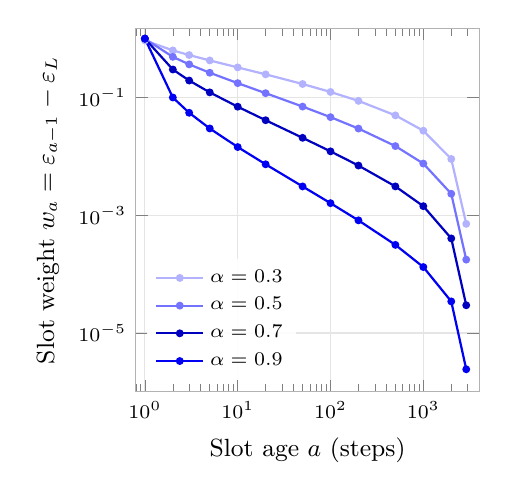
\begin{tikzpicture}
\begin{loglogaxis}[
  width=0.49\textwidth, height=6.2cm,
  xmin=0.8, xmax=4000, ymin=1e-6, ymax=1.5,
  xlabel={Slot age $a$ (steps)},
  ylabel={Slot weight $w_a = \varepsilon_{a-1}-\varepsilon_L$},
  grid=major, grid style={gray!20},
  axis line style={gray!60},
  tick label style={font=\scriptsize},
  label style={font=\small},
  legend style={font=\scriptsize, draw=none, fill=white, fill opacity=0.9, text opacity=1, at={(0.03,0.03)}, anchor=south west},
  legend cell align=left,
  every axis plot/.append style={thick, mark=*, mark size=1.0pt},
]
\addplot[color=blue!30] coordinates {(1,0.9302) (2,0.6302) (3,0.5252) (5,0.4256) (10,0.3242) (20,0.247) (50,0.1694) (100,0.1241) (200,0.08757) (500,0.04969) (1000,0.02725) (2000,0.009026) (2900,0.0007133)};
\addlegendentry{$\alpha=0.3$}
\addplot[color=blue!55] coordinates {(1,0.9897) (2,0.4897) (3,0.3647) (5,0.2631) (10,0.1752) (20,0.1183) (50,0.07009) (100,0.04633) (200,0.02967) (500,0.01495) (1000,0.007546) (2000,0.002316) (2900,0.0001762)};
\addlegendentry{$\alpha=0.5$}
\addplot[color=blue!75!black] coordinates {(1,0.9988) (2,0.2988) (3,0.1938) (5,0.1221) (10,0.06973) (20,0.04109) (50,0.02065) (100,0.01216) (200,0.006985) (500,0.003088) (1000,0.001426) (2000,0.0004041) (2900,2.957e-05)};
\addlegendentry{$\alpha=0.7$}
\addplot[color=blue!95!black] coordinates {(1,0.9999) (2,0.09992) (3,0.05492) (5,0.02976) (10,0.0144) (20,0.007331) (50,0.003085) (100,0.001602) (200,0.0008185) (500,0.000314) (1000,0.0001319) (2000,3.439e-05) (2900,2.419e-06)};
\addlegendentry{$\alpha=0.9$}
\end{loglogaxis}
\end{tikzpicture}\hfill
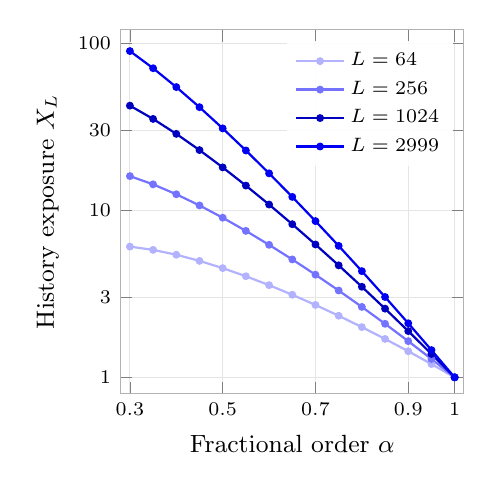
\begin{tikzpicture}
\begin{semilogyaxis}[
  width=0.49\textwidth, height=6.2cm,
  xmin=0.28, xmax=1.02, ymin=0.8, ymax=120,
  xlabel={Fractional order $\alpha$},
  ylabel={History exposure $X_L$},
  xtick={0.3,0.5,0.7,0.9,1.0},
  ytick={1,3,10,30,100},
  yticklabels={1,3,10,30,100},
  grid=major, grid style={gray!20},
  axis line style={gray!60},
  tick label style={font=\scriptsize},
  label style={font=\small},
  legend style={font=\scriptsize, draw=none, fill=white, fill opacity=0.9, text opacity=1, at={(0.97,0.97)}, anchor=north east},
  legend cell align=left,
  every axis plot/.append style={thick, mark=*, mark size=1.0pt},
]
\addplot[color=blue!30] coordinates {(0.30,6.058) (0.35,5.794) (0.40,5.418) (0.45,4.977) (0.50,4.505) (0.55,4.028) (0.60,3.563) (0.65,3.121) (0.70,2.712) (0.75,2.337) (0.80,1.999) (0.85,1.698) (0.90,1.433) (0.95,1.201) (1.00,1.000)};
\addlegendentry{$L=64$}
\addplot[color=blue!55] coordinates {(0.30,16.007) (0.35,14.287) (0.40,12.465) (0.45,10.683) (0.50,9.023) (0.55,7.526) (0.60,6.211) (0.65,5.078) (0.70,4.115) (0.75,3.309) (0.80,2.640) (0.85,2.092) (0.90,1.647) (0.95,1.288) (1.00,1.000)};
\addlegendentry{$L=256$}
\addplot[color=blue!75!black] coordinates {(0.30,42.257) (0.35,35.190) (0.40,28.648) (0.45,22.908) (0.50,18.052) (0.55,14.050) (0.60,10.819) (0.65,8.251) (0.70,6.239) (0.75,4.680) (0.80,3.485) (0.85,2.577) (0.90,1.892) (0.95,1.380) (1.00,1.000)};
\addlegendentry{$L=1024$}
\addplot[color=blue!95!black] coordinates {(0.30,89.660) (0.35,70.760) (0.40,54.592) (0.45,41.371) (0.50,30.895) (0.55,22.789) (0.60,16.629) (0.65,12.020) (0.70,8.613) (0.75,6.123) (0.80,4.321) (0.85,3.027) (0.90,2.107) (0.95,1.456) (1.00,1.000)};
\addlegendentry{$L=2999$}
\end{semilogyaxis}
\end{tikzpicture}
\caption{Left: the total forcing injected by an upset in a history slot falls as a power law in the slot's age, $w_a \approx (a^{-\alpha}-L^{-\alpha})/\Gamma(1-\alpha)$; $L = 2999$. Right: the sum of slot weights, $X_L$ (Eq.~\eqref{eq:XL}), is the history buffer's exposure per unit fluence relative to an integer-order neuron's single state register. It grows as $L^{1-\alpha}$.}
\label{fig:slots}
\end{figure}

\paragraph{Interpretation.} Two numbers describe the buffer, and they pull in opposite directions.
\begin{itemize}
  \item \textbf{Per upset.} A uniformly placed upset injects on average $X_L/(L+1)$ of what an upset in the newest sample injects: 0.010 at $\alpha = 0.5$, $L = 2999$. Most history upsets land in old slots and do almost nothing.
  \item \textbf{Per unit fluence.} With a uniform per-bit rate, each neuron's buffer receives $L+1$ times as many upsets as a single state register, so the total injected forcing per unit fluence is $X_L$ times that of an integer-order neuron: 31 at $\alpha = 0.5$ and 90 at $\alpha = 0.3$ for $L = 2999$ (Figure~\ref{fig:slots}, right).
\end{itemize}
$X_L$ is a zero-frequency measure. It counts the integrated forcing, not its time course, which the membrane and network filters shape differently for recent and old slots. It is the right first-order scaling for comparing configurations and the quantity to test first (prediction S3 in Table~\ref{tab:predictions}).

\paragraph{Large errors.} Proposition~\ref{prop:slot} is exact for any $\Delta$, but the threshold makes the response nonlinear when $\Delta$ is large. As a rough criterion, a corrupted sample keeps the neuron firing at every available step while its weight alone exceeds the gap, $|c_k|\,\Delta > V_{\mathrm{th}} - V_{\mathrm{reset}}$. That lasts up to lag
\begin{equation}
k^{*} \approx \left( \frac{\alpha\, \Delta}{\Gamma(1-\alpha)\,(V_{\mathrm{th}} - V_{\mathrm{reset}})} \right)^{1/(1+\alpha)}.
\end{equation}
For a fixed-point sign-bit flip in Q8.8 ($\Delta = 128$~mV, gap 15~mV, $\alpha = 0.5$), $k^{*} \approx 1.8$: a burst of one or two extra spikes. For an IEEE exponent flip the error is so large that the outcome is set by its sign instead:
\begin{itemize}
  \item \textbf{$\Delta > 0$.} The neuron fires on every non-refractory step until the slot is overwritten, up to $L+1-a$ steps. Reset writes $V_{\mathrm{reset}}$, so the corruption does not spread to other slots.
  \item \textbf{$\Delta < 0$}, the typical case for negative potentials (Figure~\ref{fig:bitpos}). Nothing resets the potential from below, so the next update writes a hugely negative value of its own, and the corruption propagates through the recursion like an initial condition. The neuron stays silent, and the readout sees an astronomically large value until the free response has decayed by the factor $|\Delta|/V$. For $\Delta \sim 10^{155}$ that takes hundreds of truncated time constants ($\ln 10^{155} \approx 357$). The episode is a dropout with a corrupted readout, worse than the dropout fault of~\cite{dropout2026}.
\end{itemize}
During refractory steps the update is skipped, so the forcing at those steps is lost. That is a small extra masking effect.

\subsection{Membrane potential register}

In SPIRES the update reads $V_{n-1}$ from the buffer (\texttt{V\_history[head-1]}), not from the field \texttt{V}; \texttt{V} is a copy used only by the readout. On hardware the two are one register or one memory word. An upset in the membrane potential is therefore the $a = 1$ case of Proposition~\ref{prop:slot}, applied to the buffer and its copy together. Its total forcing is $\Delta(1 - \varepsilon_L - \dta/\tau_m)$, the largest of any slot, and it also changes the readout at that step.

\subsection{Spike bits}
\label{sec:spike}

An upset in neuron $j$'s spike bit creates or deletes one spike. At the next update every postsynaptic neuron $i$ receives $\pm W_{ij}$, so its potential moves by $\pm W_{ij}\dta$. In the linear reservoir this is a forcing $\pm q_j$ for one step, and the response is
\begin{equation}
\delta(t) = \pm\, G(t - t_0)\, q_j \;\sim\; t^{-1-\alpha} \quad (t\to\infty, \text{ capped by } L).
\end{equation}
This is exactly the transient fault of~\cite{dropout2026} (their Eq.~(11)) with duration one step and amplitude $\pm1$ in place of $-s_j$. Everything said there about pulse responses carries over. In the current configuration the jump is small. With entries of standard deviation about $\rho/\sqrt{Np} \approx 0.09$ (circular law, $\rho = 0.986$, $Np \approx 123$), $|W_{ij}|\dta \approx 0.03$~mV against a 15~mV gap. So spike upsets matter only through neurons near threshold. An extra spike can then shift spike times downstream and change the spike pattern permanently even when the network is linearly stable (``stable chaos''~\cite{jahnke2008}). The right diagnostic is the spike-flip count between golden and faulty runs~\cite{dropout2026}.

In SPIRES, spikes travel between micro-steps in the local array \texttt{last\_spikes}, which is reloaded from each neuron's \texttt{spike} field only at the start of a macro-step. Injecting spike upsets inside a macro-step therefore needs a hook with access to that array (Section~\ref{sec:impl}).

\subsection{Refractory counter}
\label{sec:refrac}

On hardware the refractory period is a small counter of $n_r$ bits holding the remaining hold steps. Most of the time it is 0. An upset then sets one bit, holding the neuron at $V_{\mathrm{reset}}$ for $D = 2^{k}$ steps, where $k$ is the flipped bit. While held, the neuron emits no spikes and writes $V_{\mathrm{reset}}$ into its buffer. The event is therefore a transient dropout: the clamp fault of the existing experiment, for a duration $D$. Under a uniform choice of bit, $\log_2 D$ is uniform on $\{0, \dots, n_r - 1\}$, the same log-uniform law as Proposition~\ref{prop:loguniform}, with mean duration $(2^{n_r}-1)/n_r$ (32 steps for $n_r = 8$). The response is the dropout response of~\cite{dropout2026} truncated at $D$: a pulse of amplitude $-s_j$ and width $D$. Afterwards the buffer still holds $D$ samples of $V_{\mathrm{reset}}$, which echo through the history for up to $L$ steps.

SPIRES models the counter as a double clock \texttt{t\_prev} that grows without bound while the neuron is silent. A sign flip then holds the neuron for as long as it had been silent, and exponent flips can hold it forever. Neither behavior exists in a saturating hardware counter, so the simulation should flip a modeled $n_r$-bit counter and map it back to \texttt{t\_prev} (Section~\ref{sec:impl}).

\subsection{Buffer pointer}

The circular buffer is indexed by a pointer, \texttt{internal\_step mod mem\_len} in SPIRES. An upset shifts the pointer by $r = \pm 2^{k}$ modulo the buffer length. For the next $L+1$ steps the GL sum is applied to a cyclically rotated history, and the new writes land in slots that still hold needed samples. After $L+1$ steps every slot has been rewritten in the new order, and the buffer is consistent again. While it lasts, the error in the history sum is $\sum_k c_k (V_{n-((k+r) \bmod (L+1))} - V_{n-k})$, bounded by $(1-\varepsilon_L)\,R_V$ with $R_V$ the range of stored potentials, and dominated by the lag-1 term $\alpha(V_{n-1-r} - V_{n-1})$. On hardware the pointer is probably one counter shared by all neurons, which makes this a common-mode fault: every neuron's history is rotated at once. In SPIRES the counter is per-neuron and 64 bits wide. A flip of a high bit makes it negative or smaller than the buffer, which either indexes out of bounds or re-enters the warm-up branch and truncates the history sum. Both are simulator artifacts; the simulation must flip a modeled $\lceil\log_2(L+1)\rceil$-bit pointer instead.

\subsection{GL coefficients}
\label{sec:coeff}

All neurons share one coefficient memory~\cite{dropout2026}, and coefficients are parameters: an upset persists until the memory is scrubbed or reloaded. In SPIRES it even survives \texttt{spires\_reservoir\_reset}, which reuses the shared array. Coefficient upsets are therefore persistent and common-mode. The following result shows they can also be catastrophic.

The hardware stores $|c_k|$ for $k \ge 1$ as UQ0.16 words and subtracts. For $k \ge 2$, $|c_k| < 2^{-2}$, so its top bits are zero and flips there are $0\to1$. A flip of bit position $j$ (weight $2^{-j}$) that sets a bit raises $|c_k|$ by $2^{-j}$, which lowers $\sum_k c_k$ by $2^{-j}$. Define the leak margin
\begin{equation}
S = \varepsilon_L + \frac{\dta}{\tau_m}.
\label{eq:margin}
\end{equation}

\begin{proposition}[Coefficient upsets destabilize every neuron]
\label{prop:coeff}
If an upset lowers $\sum_{k} c_k$ by more than $S$, the subthreshold dynamics of every neuron have a real characteristic root $z^{*} > 1$ and diverge exponentially. If it lowers the sum by $\delta_c < S$, the dynamics stay stable, and the fixed point of a neuron at mean stored potential $\bar V$ moves by
\begin{equation}
\Delta \bar V = \bar V\, \frac{\delta_c}{S - \delta_c},
\label{eq:coeffshift}
\end{equation}
away from the representation's zero.
\end{proposition}
\begin{proof}
The homogeneous recursion has the characteristic function
\[
P(z) = \sum_{k=0}^{L} c'_k z^{-k} + \frac{\dta}{\tau_m}\, z^{-1},
\]
with $c'_k$ the faulty coefficients. $P(1) = S - \delta_c < 0$ and $P(z) \to c_0 = 1 > 0$ as $z\to\infty$, so $P$ has a real root in $(1,\infty)$. For the shift, the fixed point of Eq.~\eqref{eq:glflif} satisfies $\bar V\,(\sum_k c_k + \dta/\tau_m) = \dta\,(V_{\mathrm{rest}}/\tau_m + \bar I + b)$. Lowering the bracket from $S$ to $S - \delta_c$ scales $\bar V$ by $S/(S-\delta_c)$.
\end{proof}

For the current configuration ($\alpha = 0.5$, $\Delta t = 0.1$, $\tau_m = 20$, $L = 2999$), $\varepsilon_L = 0.0103$ and $\dta/\tau_m = 0.0158$, so $S = 0.026$. Any of the top 5 bits ($2^{-5} = 0.031 > S$) destabilizes the reservoir. Table~\ref{tab:coeff} gives the shift for the rest.

\begin{table}[h]
\centering
\small
\begin{tabular}{@{}cccl@{}}
\toprule
 & \multicolumn{2}{c}{$\Delta\bar V$ (mV)} & \\
\cmidrule(lr){2-3}
Bit weight $2^{-j}$ & $\bar V = -60$ mV (SPIRES) & $\bar V = 10$ mV (offset-free) & Against the 15 mV gap \\
\midrule
$2^{-1}$ to $2^{-5}$ & unstable & unstable & catastrophic \\
$2^{-6}$ & $-89$ & $14.9$ & catastrophic / marginal \\
$2^{-7}$ & $-25.6$ & $4.3$ & catastrophic / large \\
$2^{-8}$ & $-10.6$ & $1.8$ & large / moderate \\
$2^{-10}$ & $-2.3$ & $0.39$ & moderate / small \\
$2^{-12}$ & $-0.57$ & $0.09$ & small \\
$2^{-16}$ & $-0.035$ & $0.006$ & negligible \\
\bottomrule
\end{tabular}
\caption{Operating-point shift from one upset in a UQ0.16 GL coefficient, Eq.~\eqref{eq:coeffshift}, for $\alpha = 0.5$, $\Delta t = 0.1$, $\tau_m = 20$, $L = 2999$ ($S = 0.026$).}
\label{tab:coeff}
\end{table}

Three consequences.
\begin{itemize}
  \item \textbf{The voltage convention sets the failure mode and the size.} With intact coefficients $\sum_k c_k = \varepsilon_L$, and the kernel is nearly blind to constants. An upset breaks that, adding a leak (or an anti-leak) toward the representation's zero. With SPIRES' absolute potentials near $-60$~mV the extra term pushes the potential down: an unstable reservoir runs away to $-\infty$ and goes silent, and a stable one shifts toward silence. With $V_{\mathrm{rest}} = 0$ and positive potentials the same upset pushes up: the unstable reservoir fires at the maximum rate, and the shift is about six times smaller (Table~\ref{tab:coeff}).
  \item \textbf{Lower $\alpha$ is more robust here.} The truncation leak $\varepsilon_L$ grows as $\alpha$ falls, and with it the margin. For $L = 2999$ and the same $\Delta t$ and $\tau_m$: $S = 0.095$ at $\alpha = 0.3$ (top 3 bits destabilize), $0.026$ at $0.5$ (top 5), $0.011$ at $0.7$ (top 6) and $0.0064$ at $0.9$ (top 7). An integer-order design has no coefficient memory and no such vulnerability.
  \item \textbf{The network is more fragile than one neuron.} In the linear reservoir, $\dta/\tau_m$ in Eq.~\eqref{eq:margin} becomes $-\dta\lambda_r$, with $\lambda_r$ the rightmost real eigenvalue of $A$. Recurrent excitation moves $\lambda_r$ above $-1/\tau_m$ and shrinks the margin. Near the edge of stability the margin is $\varepsilon_L$ alone.
\end{itemize}
The dynamic effect depends on the lag $k$ of the corrupted coefficient: it adds $\delta_c z^{-k}$ to the kernel $C_L(z)$, a delayed self-feedback of gain $\delta_c$ at lag $k$. But the DC effect, which decides stability, depends only on the total.

Because $|c_k|$ is strictly decreasing in $k$ for $0 < \alpha < 1$, any upset large enough to matter breaks monotonicity. A comparator check $|c_k| \le |c_{k-1}|$ on each read detects every destabilizing upset, for the cost of one comparison per coefficient.

\subsection{Recurrent weights}
\label{sec:weights}

A weight upset changes $W_{ij}$ by $\delta_w$ and persists until scrubbed. In the linear reservoir it is a rank-one change $\Delta A = \delta_w \gamma_j\, e_i e_j^{\top}$. By the matrix determinant lemma, the eigenvalues $\mu$ of the faulty reservoir solve
\begin{equation}
1 = \delta_w\, \gamma_j \left[ (\mu \mathrm{Id} - A)^{-1} \right]_{ji},
\label{eq:secular}
\end{equation}
which gives the exact spectral effect of a single weight upset, not only the first-order bound of~\cite{dropout2026}. Stability is lost if a root enters Matignon's sector $|\arg\mu| \le \alpha\pi/2$. The mean drive into neuron $i$ changes by $\delta_w r_j$, shifting the operating point by $\delta^{*} = -A^{-1} e_i\, \delta_w r_j$ (replace $A$ by $A - (\varepsilon_L/\dta)\,\mathrm{Id}$ for a truncated buffer).

The size of $\delta_w$ follows Proposition~\ref{prop:loguniform}, so most weight upsets are tiny. A sign-bit or top-bit upset is not: it can make one synapse larger than the gap, $|W_{ij} + \delta_w|\,\dta > V_{\mathrm{th}} - V_{\mathrm{reset}}$. Every spike of $j$ then forces a spike in $i$ (a relay synapse) or, if inhibitory, silences $i$. A sign flip also breaks Dale's law. The storage backend changes the target:
\begin{itemize}
  \item \textbf{Dense storage} keeps $N^2$ words, including zeros. An upset in a zero creates a new synapse, a structural fault.
  \item \textbf{Sparse (CSR) storage} keeps only the $\mathrm{nnz}$ existing weights but adds index fields. An upset in a column index moves a synapse to another presynaptic neuron, $\Delta W = W_{ij}(e_i e_{j'}^{\top} - e_i e_j^{\top})$ with $j' = j \oplus 2^{k}$. An upset in a row pointer moves a whole block of synapses between neighbouring rows, or makes a row's range empty or negative.
\end{itemize}
SPIRES should store weights in the same backend as the hardware, or the fault population is wrong.

\subsection{Input weights and input gain}

An upset in $W^{\mathrm{in}}_{im}$ adds an input-correlated forcing $e_i\,\delta\, u_m(t)$ to neuron $i$ until scrubbed: an extra, miscalibrated input channel. The input gain (\texttt{input\_strength} in SPIRES) is a single shared register that scales all of $B$. An upset there changes the drive of every neuron at once, shifting the whole operating point, a common-mode fault in one word.

\subsection{Readout weights}
\label{sec:readout}

A readout upset does not touch the dynamics. With a fixed readout it adds the output error $e(t) = \delta_w\, x_j(t)$ until scrubbed, which splits into a bias $\delta_w \bar x_j$ and a fluctuation $\delta_w \tilde x_j$. Since SPIRES reads absolute potentials and has no intercept, the bias is large, $\delta_w \times (\approx -60~\mathrm{mV})$.

With online LMS learning the readout repairs itself, but unevenly. To first order, under the usual independence assumption~\cite{widrow1985}, the weight error evolves as
\begin{equation}
\E[\delta w_{t+1}] = \left( \mathrm{Id} - \mu_{\mathrm{lr}}\, R \right) \E[\delta w_t], \qquad R = \E[x x^{\top}] = C + \bar x \bar x^{\top}.
\end{equation}
The component along the mean direction $\bar x$ decays at rate $\mu_{\mathrm{lr}}\|\bar x\|^2$ per step. For $N = 400$, $\bar x \approx -57$~mV and $\mu_{\mathrm{lr}} = 10^{-7}$ that is about 0.13, so the bias is removed within about ten steps. Components in the fluctuation subspace decay at $\mu_{\mathrm{lr}} \lambda_i(C)$, orders of magnitude slower when $\lambda_i(C) \ll \|\bar x\|^2$. Online learning at this rate therefore corrects the bias of a readout upset, but not the input-carrying part of the error.

Online learning also works in the other direction. A transient state upset changes $x(t)$, and the LMS update $\mu_{\mathrm{lr}}\, e(t)\, x(t)$ writes it into the weights, where it persists. In fixed point the damage is bounded. In binary64 an exponent flip in the state makes the update overflow, the weights become NaN, and every later output is NaN. With online learning on, a transient fault can become a permanent one.

\subsection{Datapath transients}
\label{sec:set}

The GL update is a long multiply-accumulate over $L$ products, the largest combinational block in the design. A latched transient in it corrupts one computed $V_{i,n}$ before it is written. That has the effect of an $a = 1$ history upset at the moment of writing, plus a possibly wrong spike decision, since the threshold comparison sees the corrupted value. Its rate is set by datapath size and clock frequency (Eq.~\eqref{eq:platch}), not by storage size. For a time-multiplexed design, where one update unit serves all neurons in turn, the rate per neuron is the unit's rate divided by $N$.

\subsection{Configuration memory, functional interrupts and latch-up}
\label{sec:config}

\begin{itemize}
  \item \textbf{Configuration upsets} in an SRAM FPGA change look-up-table contents or routing until scrubbed~\cite{quinn2005,amd_sem}. Only a fraction of configuration bits are essential to the design, and the functional effect of each depends on the placed-and-routed netlist, which a software simulator does not have. Two approximations bracket it: a persistent stuck-at fault on one datapath bit of one neuron's update for the scrub interval, and the dropout fault of~\cite{dropout2026} for the same interval. In a time-multiplexed design the affected unit serves every neuron, and the fault is common-mode. Faithful configuration studies need hardware injection (Section~\ref{sec:hil}).
  \item \textbf{Functional interrupts} hang or reset the controller. They are modeled as a freeze (no updates, output held) of duration $D$, or as a full state reset followed by warm-up from an empty history.
  \item \textbf{Latch-up} forces a power cycle: total outage, loss of all state, and a warm-up afterwards. If it damages the device, the affected region drops out permanently.
\end{itemize}
A stuck-at fault forces bit $k$ to $b^{*}$: $x \to x + (b^{*} - b_k(x))\,2^{k-F}$, re-applied after every write, so it depends on the value and persists.

\subsection{Summary: every class as a forcing}

Table~\ref{tab:forcing} summarizes the classes in the language of~\cite{dropout2026}. The neuron-output faults (spike, refractory, configuration, dropout) differ only in amplitude and duration along the same direction $q_j$. In the linear regime, faults with the same integrated forcing have the same far-field effect. That gives a principled way to compare radiation upsets with neuron dropout (research question 3 of the thesis plan): match them on integrated forcing, or on physical rate (Section~\ref{sec:fluence}).

\begin{table}[h]
\centering
\small
\begin{tabularx}{\textwidth}{@{}l>{\raggedright\arraybackslash}X>{\raggedright\arraybackslash}p{3.0cm}>{\raggedright\arraybackslash}p{3.1cm}@{}}
\toprule
Class & Equivalent perturbation & Duration & Tail (linear model) \\
\midrule
History slot, age $a$ & Forcing comb $\Delta|c_{a+m}|$ on neuron $i$, total $\Delta w_a$ & $L+1-a$ steps & $t^{-1-\alpha}$, capped by $L$ \\
Membrane potential & Same with $a = 1$; plus one readout error & $L$ steps & as above \\
Spike bit & Forcing $\pm q_j$ & 1 step & $t^{-1-\alpha}$ \\
Refractory counter & Dropout of $j$: forcing $-q_j s_j$, readout sees $V_{\mathrm{reset}}$ & $2^{k}$ steps & $t^{-1-\alpha}$ after release \\
Buffer pointer & Rotated history, all neurons if shared & $L+1$ steps & as history \\
GL coefficient & Kernel $C_L(z) + \delta_c z^{-k}$, all neurons & until scrub & step; unstable if $\delta_c > S$ \\
Recurrent weight & Rank-one $\Delta A$ and mean drive $\delta_w r_j$ & until scrub & step, then $t^{-1-\alpha}$ \\
Input weight, gain & Forcing $\delta\,u(t)$; gain: all neurons & until scrub & step \\
Readout weight & Output error $\delta_w x_j(t)$ & until scrub & none (no dynamics) \\
Configuration & Stuck datapath bit, or dropout & until scrub & step, then $t^{-1-\alpha}$ \\
\bottomrule
\end{tabularx}
\caption{Fault classes as perturbations of the reservoir.}
\label{tab:forcing}
\end{table}

%=====================================================================
\section{The reservoir's response}
\label{sec:response}

\subsection{Transient and persistent faults}

The two persistence classes have different recovery laws, both derived from the results of~\cite{dropout2026}.
\begin{itemize}
  \item \textbf{Transient (state) upsets} are pulses. The response is the impulse response $G$, with a $t^{-1-\alpha}$ tail that turns exponential near $L$. The tail is integrable, so each transient upset costs finite cumulative error.
  \item \textbf{Persistent (parameter) upsets} are steps that switch on at $t_f$ and off at the next scrub, $t_f + T_s$. In the linear reservoir, with mode forcing $F$ and the step response $\delta^{*}[1 - E_\alpha(\lambda t^\alpha)]$,
  \begin{equation}
  \delta(t) = \delta^{*}\left[ E_\alpha\!\left(\lambda (t - t_f - T_s)^{\alpha}\right) - E_\alpha\!\left(\lambda (t-t_f)^{\alpha}\right) \right] \approx F\, T_s\, G(t - t_f) \quad (t - t_f \gg T_s).
  \label{eq:scrubtail}
  \end{equation}
  After repair the reservoir remembers the faulty episode, and it forgets it with the same $t^{-1-\alpha}$ tail as a transient fault of duration $T_s$. The approximation uses $\frac{d}{dt}[1 - E_\alpha(\lambda t^\alpha)] = -\lambda t^{\alpha-1}E_{\alpha,\alpha}(\lambda t^\alpha)$ and $\delta^{*} = -F/\lambda$. The outage of a persistent upset is therefore its exposure (mean $T_s/2$) plus the recovery time $T_{1\%}$ of~\cite{dropout2026} (their Eq.~(13)).
\end{itemize}

\subsection{Beyond the linear regime}

Large upsets push neurons across threshold, which the linear theory does not capture: threshold crossings, cascades with branching ratio $m$, and the deafened-but-firing behavior described in~\cite{dropout2026} all apply. Two effects are specific to upsets. First, the log-uniform error law means every class contains both negligible and maximal errors, so the response to a class is a mixture of a linear regime (most upsets) and a nonlinear one (a few). Average effects are dominated by the few, which is why outcomes should be stratified by bit position (Section~\ref{sec:metrics}). Second, spike-pattern divergence after small upsets (stable chaos) means that matching the exact spike train of the golden run is the wrong success criterion. The criterion should be task-level: output error and recovery of the readout.

\subsection{Comparing configurations at equal fluence}
\label{sec:fluence}

Equation~\eqref{eq:factor} makes the fair comparison explicit. Two reservoirs in the same environment see the same per-bit rate $\lambda$, not the same number of upsets. Their failure rates are $\lambda \sum_c N_c \AVF_c$, which differ through $N_c$ as well as through $\AVF_c$. The existing experiment fires a fixed number of faults per step, so it compares $\AVF$-like quantities and silently normalizes the target size away. That answers ``which reservoir tolerates a given upset better?'' It does not answer ``which reservoir fails less often in a radiation environment?'' For history upsets, Proposition~\ref{prop:exposure} predicts the answer to the second question to first order: total injected forcing per unit fluence scales as $X_L \propto L^{1-\alpha}$, against 1 for integer order. A fractional reservoir must therefore be $X_L$ times more tolerant per unit of injected forcing to break even. Both questions are worth answering, and the thesis should state which one each experiment addresses.

%=====================================================================
\section{Measuring vulnerability}
\label{sec:metrics}

\subsection{Outcomes and metrics}

Each injected upset is compared with a golden run that shares its input and its history up to the injection time. With $e(t) = y'(t) - y(t)$ the output difference over a horizon $H$:
\begin{itemize}
  \item \textbf{Outcome class.} \emph{Masked}: $|e(t)| < \epsilon_{\mathrm{tol}}$ throughout. \emph{Transient}: above tolerance, but below it again within $H$. \emph{Persistent}: still above tolerance at $H$. \emph{Catastrophic}: non-finite output, silence or saturation of the reservoir.
  \item \textbf{Per-event metrics.} Peak error $\max_t |e(t)|$; error energy $\sum_t e(t)^2$; recovery time $T_\epsilon$; spike-flip count; and, for history upsets, the slot age $a$ and value error $\Delta$, so that results can be checked against Proposition~\ref{prop:slot}.
\end{itemize}
$\AVF_c$ is then the fraction of non-masked outcomes, or of outcomes above a task-relevant error-energy threshold. The horizon must be long enough to see recovery: several $L$ micro-steps, not the 10 macro-steps used so far.

\subsection{How many injections}

Statistical fault injection~\cite{leveugle2009} estimates a proportion $p$ from $n$ injections drawn from a population of $N_{\mathrm{pop}}$ (bit, time) pairs. For margin $e$ at confidence quantile $t$,
\begin{equation}
n = \frac{N_{\mathrm{pop}}}{1 + e^2 (N_{\mathrm{pop}} - 1)/(t^2 p(1-p))} \;\approx\; \frac{t^2\, p(1-p)}{e^2},
\label{eq:samplesize}
\end{equation}
which for the worst case $p = 0.5$ and 95\% confidence gives 9604 injections for $\pm1\%$, 2401 for $\pm2\%$ and 384 for $\pm5\%$. For small $p$, report Wilson intervals~\cite{wilson1927} rather than normal ones.

Uniform sampling wastes almost all of its budget. History bits are 94\% of the population, and most of their upsets are masked, while the rare catastrophic outcomes (coefficient MSBs, exponent bits) sit in strata that uniform sampling barely visits. Stratify by class and by bit position. With stratum weights $w_s$ (the stratum's share of $\lambda N$) and $n_s$ injections per stratum, the combined estimate $\hat p = \sum_s w_s \hat p_s$ has variance $\sum_s w_s^2 p_s(1-p_s)/n_s$, which Neyman allocation, $n_s \propto w_s\sqrt{p_s(1-p_s)}$, minimizes for a fixed total. A small pilot run supplies the $p_s$. Small strata can be covered exhaustively: the pointer (12 bits), the input gain (16 bits) and the coefficient MSBs ($3000 \times 5$ bits). For those, injection time is the only random dimension.

\subsection{Fluence--response and mission metrics}

Two kinds of experiment complement the single-upset campaign.
\begin{itemize}
  \item \textbf{Fluence--response curves.} Run with Poisson upsets at increasing acceleration and plot a task metric against fluence $\Phi$ (or expected upsets per bit). The slope at the origin is the system cross section, $\sigma_{\mathrm{sys}} = \sum_c \sigma_c N_c \AVF_c$. The departure from linearity measures fault interaction. This is the software analogue of a beam test.
  \item \textbf{Mission metrics.} From Eq.~\eqref{eq:factor}: the mean time to failure, $1/\Lambda_{\mathrm{fail}}$; the reliability, $\exp(-\Lambda_{\mathrm{fail}}t)$; and the unavailability, $U \approx \sum_c \lambda_c N_c \AVF_c\, \E[\mathrm{outage}_c]$, with outage $T_{\mathrm{rec}}$ for transient classes and $T_s/2 + T_{\mathrm{rec}}$ for persistent ones.
\end{itemize}

%=====================================================================
\section{Mitigation, briefly}
\label{sec:mitigation}

Mitigation is not the thesis's subject, but a reservoir's intrinsic tolerance only means something compared with the cost of standard protection. The results above suggest where protection pays.
\begin{itemize}
  \item \textbf{Protect the common-mode words first.} Coefficients, buffer pointer and input gain are a tiny fraction of the bits but produce the reservoir-wide failures. SEC-DED with scrubbing (Eq.~\eqref{eq:secded}) or TMR on these costs almost nothing.
  \item \textbf{Protect the top bits, not whole words.} By Proposition~\ref{prop:loguniform}, protecting the top $j$ bits of each word leaves $4^{-j}$ of the mean square error.
  \item \textbf{Use invariants the model provides.} Stored potentials lie in a known range, and coefficients are monotone. Range and monotonicity checks catch all large upsets, including every destabilizing coefficient upset (Section~\ref{sec:coeff}).
  \item \textbf{Store offset-free.} With $V_{\mathrm{rest}} = 0$, coefficient and readout upsets act on deviations from rest rather than on absolute potentials.
  \item \textbf{The readout can repair itself, partially.} Online learning corrects the bias part of readout upsets quickly (Section~\ref{sec:readout}). It should be paired with range checks, or it will learn transient faults into the weights.
\end{itemize}
On FPGAs, configuration scrubbers such as AMD's SEM controller~\cite{amd_sem} repair configuration memory but not block-RAM contents, which need the block RAM's own ECC.

%=====================================================================
\section{Testable predictions}

\begin{table}[h]
\centering
\small
\begin{tabularx}{\textwidth}{@{}l>{\raggedright\arraybackslash}X>{\raggedright\arraybackslash}X>{\raggedright\arraybackslash}X@{}}
\toprule
\# & Prediction & How to test & What would falsify it \\
\midrule
S1 & Binary64 injection overstates catastrophic outcomes relative to fixed point; in fixed point, mean square damage is dominated by the top bit & Same campaign in both formats, stratified by bit (E1) & Similar catastrophic rates, or damage spread evenly over bits \\
S2 & In the linear regime, history-upset damage scales with $w_a = \varepsilon_{a-1}-\varepsilon_L$: log--log slope $-\alpha$ in age, cutoff at $L$ & Bin history injections by age; small $\Delta$ (E2) & Slope independent of $\alpha$ \\
S3 & Per unit fluence, history-induced error scales with $X_L \propto L^{1-\alpha}$ & Equal-fluence runs across $\alpha$ and $L$ (E4) & Error independent of $L$ at fixed $\alpha<1$ \\
S4 & A coefficient upset destabilizes the reservoir iff it lowers $\sum c_k$ by more than $S$ (network: by more than $\varepsilon_L - \dta\lambda_r$); the critical bit moves down as $\alpha$ rises & Exhaustive coefficient-MSB injection across $\alpha$ (E3) & Instability below the margin, or none above it \\
S5 & Coefficient-upset shifts and readout-upset bias scale with the distance of stored values from the representation's zero & Repeat S4 and readout injections with $V_{\mathrm{rest}} = 0$ (E3, E6) & Same damage with both conventions \\
S6 & Spike-bit upsets give the linear pulse response with a $t^{-1-\alpha}$ tail; nonlinear damage only through near-threshold neurons & Compare with the linear reservoir; regress damage on threshold distance (E2) & Damage uncorrelated with threshold distance \\
S7 & A persistent upset scrubbed after $T_s$ costs exposure $T_s/2$ plus $T_{1\%}$, and leaves a $t^{-1-\alpha}$ tail & Sweep $T_s$ (E5) & Post-scrub error decaying exponentially from the start \\
S8 & Online LMS removes the bias of a readout upset within $\sim 1/(\mu_{\mathrm{lr}}\|\bar x\|^2)$ steps, not the fluctuation; with binary64 state upsets it turns transient faults into permanent NaN readouts & Readout and state injections, online on and off (E6) & Fluctuation error removed at the bias rate \\
S9 & At matched integrated forcing, spike, refractory and dropout faults on neuron $j$ have the same far-field effect in the linear regime & Matched-forcing comparison (E7) & Effects that differ beyond the nonlinear corrections \\
\bottomrule
\end{tabularx}
\caption{Predictions for the single-event-effect experiments.}
\label{tab:predictions}
\end{table}

%=====================================================================
\section{Implementation plan for SPIRES}
\label{sec:impl}

The plan targets the upstream SPIRES tree (\href{https://github.com/txmastin/spires}{txmastin/spires}, \texttt{main} at commit 43ab33f). The fault-injection version used for the dropout experiments lives on another system. It should be merged first, so that the new fault classes extend its seeded fault system (the four-argument \texttt{spires\_create\_fault\_system} that the Mackey--Glass experiment calls) rather than duplicating it. Everything below adds new code beside it and changes the existing core in only four places.

\subsection{Design requirements}

\begin{enumerate}
  \item \textbf{Hardware-faithful errors.} Every class carries the hardware's number format and offset. Upsets are applied with Eq.~\eqref{eq:delta}. Counters and pointers are modeled at hardware width.
  \item \textbf{Reproducible.} The fault realization is a pure function of a fault seed, independent of the reservoir seed and of training, as in the existing experiment. Use a dedicated \texttt{spires\_rng} stream; never the global \texttt{rand()}.
  \item \textbf{Free when off.} With no fault system attached, outputs are bit-identical to stock SPIRES, and the cost is one null-pointer test per micro-step.
  \item \textbf{Micro-step resolution.} Upsets land between micro-steps, at the moment the hardware's registers hold their values.
  \item \textbf{Paired runs.} Golden and faulty runs share input and history up to the injection, and a campaign can restart from snapshots instead of re-running warm-up.
\end{enumerate}

\subsection{Changes to the existing core}

\begin{enumerate}
  \item \textbf{A micro-step hook in \texttt{step\_reservoir}} (\texttt{src/reservoir.c}). It is called at the top of each micro-step, before \texttt{synapse\_prepare}, single-threaded, outside the OpenMP region. It can modify \texttt{last\_spikes}, and it returns flags asking for the input projection to be recomputed after a \texttt{W\_in} or gain upset:
\begin{lstlisting}
for (int t = 0; t < num_micro_steps; t++) {
    if (r->fault_hook) {
        unsigned dirty = r->fault_hook(r, last_spikes, r->fault_ctx);
        if (dirty & FAULT_DIRTY_INPUT)
            cblas_dgemv(CblasRowMajor, CblasNoTrans, num_neurons, num_inputs,
                        r->input_strength, r->W_in, num_inputs,
                        input_vector, 1, 0.0, external_inputs, 1);
    }
    const double *effective_input = synapse_prepare(&r->W, last_spikes, r->dt);
    /* ... unchanged ... */
    r->micro_step++;
}
\end{lstlisting}
  \item \textbf{Fields in \texttt{struct reservoir}} (\texttt{src/reservoir.h}): \texttt{fault\_hook}, \texttt{fault\_ctx} and a global \texttt{micro\_step} counter, which \texttt{reset\_reservoir} zeroes.
  \item \textbf{Weight accessors in the synapse layer} (\texttt{src/synapse.c}, \texttt{src/synapses/simple.c}). The synapse matrix is opaque, so add three accessors:
  \begin{center}\texttt{synapse\_values()},\quad \texttt{synapse\_col\_idx()},\quad \texttt{synapse\_row\_ptr()}.\end{center}
  They return pointers and lengths for \texttt{SYNAPSE\_SIMPLE} on either backend, and \texttt{NULL} for the other synapse types, whose weight classes are then disabled with a warning.
  \item \textbf{State snapshot and restore} (\texttt{src/reservoir.c}): copy each GL neuron's \texttt{V}, \texttt{spike}, \texttt{t\_prev}, \texttt{internal\_step} and \texttt{V\_history}, plus \texttt{micro\_step}. Refuse stateful synapse types and plasticity for now. A snapshot of the current configuration is about 10~MB.
\end{enumerate}

\subsection{The new module}

The module lives in \texttt{src/see/}, five small files with one job each.

\paragraph{\texttt{format.c}: number formats.} Implements Eq.~\eqref{eq:delta} for three kinds: the native binary64 (bit-cast flip), binary32 (flip in the float, add the difference) and fixed point (width, fractional bits, signedness, offset, saturating encode, wrapping decode).
\begin{lstlisting}
typedef enum { SPIRES_FMT_NATIVE64, SPIRES_FMT_IEEE32, SPIRES_FMT_FIXED } spires_fmt_kind;

typedef struct {
    spires_fmt_kind kind;
    int    bits;       /* W, for FIXED */
    int    frac_bits;  /* F */
    int    is_signed;  /* two's complement if nonzero */
    double offset;     /* stored = round((x - offset) * 2^F) */
} spires_num_format;

/* x plus the error the hardware word sees when the bits in mask flip. */
double see_flip(double x, const spires_num_format *f, uint64_t mask);
/* x with bit k forced to b, for stuck-at faults. */
double see_stuck(double x, const spires_num_format *f, int k, int b);
\end{lstlisting}

\paragraph{\texttt{targets.c}: the target registry.} One entry per class of Table~\ref{tab:inventory}, built from the reservoir when the fault system is created. Each entry records the word count, bits per word, format, scope (per neuron or shared), persistence and a pair of accessors that read and write word $w$. The class-specific mappings onto SPIRES are where the subtleties of Section~\ref{sec:classes} live:
\begin{itemize}
  \item \textbf{Membrane potential:} slot $(\texttt{internal\_step}-1) \bmod \texttt{mem\_len}$ of \texttt{V\_history}, with \texttt{V} updated to the same value.
  \item \textbf{History:} word $w = i \cdot \texttt{mem\_len} + s$ is slot $s$ of neuron $i$. Log the slot's age $a$ with the event. If $s$ is the newest slot, update \texttt{V} too.
  \item \textbf{Spike:} toggle \texttt{last\_spikes[j]} (the bit in transit), not the neuron's \texttt{spike} field.
  \item \textbf{Refractory:} convert \texttt{t\_prev} to an $n_r$-bit count of remaining hold steps, $r = \max(0, \lceil (t_{\mathrm{ref}} - \texttt{t\_prev})/dt \rceil)$. Flip it, then map back with half-step offsets, $\texttt{t\_prev} = t_{\mathrm{ref}} - (r' - \tfrac12)\,dt$ (or $t_{\mathrm{ref}} + \tfrac12 dt$ for $r' = 0$), which avoids the floating-point accumulation issue of the refractory clock noted in~\cite{dropout2026}.
  \item \textbf{Pointer:} convert to a $\lceil\log_2 \texttt{mem\_len}\rceil$-bit pointer $p$. Flip it; if $p' \ge \texttt{mem\_len}$, apply the configured policy (wrap by default). Set $\texttt{internal\_step} \mathrel{+}= p' - p$, keeping it at least \texttt{mem\_len} so the warm-up branch is not re-entered. With \texttt{shared\_pointer} set, apply the same $p'$ to all neurons, which are in lockstep.
  \item \textbf{Coefficients:} words $k = 1,\dots,L$ of the shared array, flipped as UQ0.$F$ magnitudes. Keep a golden copy: \texttt{spires\_reservoir\_reset} does not restore it.
  \item \textbf{Weights and indices:} through the new accessors. Column-index upsets that leave $[0, N)$ follow a policy: wrap, or drop the synapse until scrubbed.
  \item \textbf{Input weights, gain, readout:} direct arrays. Raise \texttt{FAULT\_DIRTY\_INPUT} for the first two.
\end{itemize}

\paragraph{\texttt{events.c}: the arrival process.} It draws the next arrival time from an exponential with mean $1/\mu$ micro-steps (Eq.~\eqref{eq:mu}), so its cost is per upset, not per step. Classes are chosen with probabilities $\pi_c$ (Eq.~\eqref{eq:pic}), using an alias table. Each event is expanded into a cluster (geometric size, interleave factor $I$) and its flips are applied. Time-varying rates use thinning. An explicit mode applies a list of (class, word, bit, micro-step) records instead, which is what campaigns use and what can be replayed on hardware.
\begin{lstlisting}
static unsigned see_hook(struct reservoir *r, double *spikes, void *ctx)
{
    struct see *s = ctx;
    unsigned dirty = 0;
    see_apply_scheduled(s, r, spikes, &dirty);          /* explicit list */
    if (s->scrub_period && r->micro_step % s->scrub_period == s->scrub_phase)
        see_scrub(s, r, &dirty);
    while (s->next_arrival <= r->micro_step) {          /* Poisson stream */
        int c = alias_draw(&s->classes, &s->rng);
        uint64_t bit = rng_below(&s->rng, s->bits[c]);
        see_apply_cluster(s, r, c, bit, spikes, &dirty); /* MCU + log */
        s->next_arrival += see_exp_steps(&s->rng, s->mu);
    }
    return dirty;
}
\end{lstlisting}

\paragraph{\texttt{scrub.c}: repair.} Golden copies of the persistent classes. A scrub either restores everything (configuration-style) or applies SEC-DED semantics word by word: compare encoded current and golden words, correct a Hamming distance of 1, and log distances of 2 or more as detected-uncorrectable. Online learning writes the readout legitimately, so the training call must refresh the readout's golden copy after each update.

\paragraph{\texttt{log.c}: the event log.} One record per flipped bit: micro-step, class, word, neuron, bit, slot age, value before and after, cluster id. Written as CSV, it is both the analysis input and the fault list for hardware replay.

\paragraph{Public API} (\texttt{include/spires.h}), next to the existing fault-system calls:
\begin{lstlisting}
typedef struct {
    double   rate_per_bit;               /* upsets per bit per micro-step, incl. K */
    spires_num_format fmt[SPIRES_SEE_NUM_CLASSES];
    double   class_weight[SPIRES_SEE_NUM_CLASSES]; /* relative sigma; 0 = off */
    double   mcu_theta;  int interleave; /* cluster model */
    long     scrub_period; int ecc;      /* repair model */
    int      shared_pointer; int refrac_bits;
    uint64_t seed;
} spires_see_config;

spires_status spires_see_create(spires_reservoir *r, const spires_see_config *cfg,
                                spires_see **out);
spires_status spires_see_attach(spires_reservoir *r, spires_see *s);
spires_status spires_see_detach(spires_reservoir *r);
spires_status spires_see_schedule(spires_see *s, spires_see_class c, size_t word,
                                  int bit, uint64_t micro_step);
spires_status spires_see_scrub(spires_see *s);
size_t        spires_see_bit_count(const spires_see *s, spires_see_class c);
spires_status spires_see_write_log(const spires_see *s, const char *path);
void          spires_see_destroy(spires_see *s);

spires_status spires_snapshot_take(const spires_reservoir *r, spires_snapshot **out);
spires_status spires_snapshot_restore(spires_reservoir *r, const spires_snapshot *s);
\end{lstlisting}

\subsection{Experiment drivers}

\paragraph{Single-upset campaign.} Estimates $\AVF_c$ and the conditional error distributions.
\begin{enumerate}
  \item \textbf{Golden run.} Warm up, then run the evaluation window. Store a snapshot every $K_s$ macro-steps, the outputs at every step and the states and spikes subsampled.
  \item \textbf{For each injection} drawn by the stratified allocation (class, bit position, word, micro-step):
  \begin{enumerate}
    \item Restore the nearest earlier snapshot and run fault-free to the injection step.
    \item Schedule the upset and run $H$ macro-steps.
    \item Compare with the golden outputs; record outcome, metrics and event record.
    \item Restore the persistent classes from their golden copies.
  \end{enumerate}
\end{enumerate}
Injections are independent and run in parallel across cluster jobs. At the current size a micro-step costs about $NL \approx 1.2\times10^6$ multiply-accumulates for the history alone. Each injection with $H$ of a few thousand macro-steps takes seconds, and $10^4$ injections take node-hours to tens of node-hours. Exploratory runs can use a smaller $L$.

\paragraph{Mission and fluence runs.} Poisson upsets at acceleration $K$, scrubbing on, run long. Record the task metric against cumulative fluence and the event log. Repeat over fault seeds at fixed reservoir seeds, so that fault realizations are paired across configurations, as in the existing baseline sweep.

\paragraph{The Mackey--Glass experiment.} The driver, \texttt{faulty\_mackey\_glass\_experiment.c}, gets a fault mode \texttt{see}, with command-line arguments for the per-bit rate, class mask, format specification and scrub period. Keep the \texttt{RESULT} line and append outcome counts. Three changes to the existing protocol are needed for these measurements:
\begin{itemize}
  \item The series (1000 macro-steps) is only about three buffer lengths ($L\,dt = 300$ macro-steps). Lengthen it so that the evaluation window spans several recovery times after a washout that is excluded from the metrics.
  \item Scale the post-fault window (now 10 macro-steps) with $L$.
  \item Report non-finite outputs as a catastrophic outcome rather than letting them turn the RMSE into NaN.
\end{itemize}
One check on the other system: upstream \texttt{init\_flif\_gl} reads eight parameters (it added \texttt{t\_ref} as \texttt{params[7]}), while the experiment passes a seven-element array. If the modified library has picked up that change, the eighth read is out of bounds.

\subsection{Verification}

Each check has an exact expected result, so failures point at the code, not the theory.
\begin{enumerate}
  \item \textbf{Formats.} Encode--decode round trips; flipping bit $k$ in fixed point changes the value by exactly $\pm2^{k-F}$; native flips equal bit-casts; binary32 flips match \texttt{float} arithmetic.
  \item \textbf{Zero-rate regression.} With the fault system attached at rate 0, outputs are bit-identical to an unattached run.
  \item \textbf{History identity.} A single neuron without threshold reproduces Eq.~\eqref{eq:slotarea} to round-off for several slot ages and $\alpha$ values. It passed in the standalone simulation reported in Section~\ref{sec:history}; it should become a test in the suite.
  \item \textbf{Coefficient threshold.} Upsets just above and below the margin $S$ diverge and do not, respectively; below it, the shift matches Eq.~\eqref{eq:coeffshift}.
  \item \textbf{Spike, refractory and pointer.} A spike upset in a thresholdless linear network gives $\pm\dta G q_j$. A refractory upset of bit $k$ holds the neuron for exactly $2^{k}$ steps. A pointer upset leaves the buffer consistent after $L+1$ steps.
  \item \textbf{Arrival process.} Counts per window have dispersion index 1; class frequencies pass a $\chi^2$ test against $\pi_c$; cluster sizes match the geometric law.
  \item \textbf{Determinism and memory safety.} Identical logs and outputs with 1 and 8 OpenMP threads. Address and undefined-behavior sanitizers clean under index and pointer campaigns.
\end{enumerate}

\subsection{Experiments}

\begin{enumerate}[label=E\arabic*.]
  \item \textbf{Format.} Bit-position vulnerability maps per class, in binary64 and in the hardware's fixed-point formats (S1).
  \item \textbf{History and spikes.} Damage against slot age and $\Delta$, against $\alpha$ (S2); spike-upset damage against threshold distance (S6).
  \item \textbf{Shared words.} Exhaustive coefficient-MSB, pointer and gain campaigns across $\alpha$ and both voltage conventions (S4, S5).
  \item \textbf{Equal fluence.} Fluence--response curves across $\alpha$ and $L$ at a common per-bit rate, compared with the equal-probability design of the existing sweep (S3).
  \item \textbf{Scrubbing.} Persistent upsets with a sweep of $T_s$; exposure, recovery and post-scrub tails (S7).
  \item \textbf{Readout and online learning.} Readout and state upsets with online learning on and off (S5, S8).
  \item \textbf{Upsets versus dropout.} Spike, refractory and dropout faults on the same neurons, matched on integrated forcing and on physical rate (S9; thesis question 3).
\end{enumerate}

\subsection{Hardware cross-validation}
\label{sec:hil}

The event log doubles as a hardware fault list. On the HiL rig the same (class, word, bit, cycle) records can be applied by flipping block-RAM or register bits through the debug interface, and configuration upsets through the SEM controller's injection port~\cite{amd_sem}. Comparing $\AVF_c$ per class between simulation and hardware validates the format and inventory assumptions. Configuration upsets can only be measured there. Before the campaign, the following must be confirmed from the FPGA design, since every result above depends on them:
\begin{itemize}
  \item the word formats and offsets of potentials, history, weights and coefficients;
  \item whether coefficients sit in block RAM or in LUT-ROM (configuration memory);
  \item whether the buffer pointer is shared;
  \item whether neuron updates are parallel or time-multiplexed;
  \item the refractory counter width;
  \item whether block-RAM ECC and configuration scrubbing are enabled;
  \item the clock rate and cycles per micro-step (for Eq.~\eqref{eq:mu}).
\end{itemize}

\subsection{Order of work}

\begin{enumerate}
  \item Merge the fault-injection version from the other system onto upstream \texttt{main}, and apply the protocol changes to the Mackey--Glass experiment.
  \item Core changes (hook, accessors, snapshots) and the format layer, with verification items 1--2.
  \item Target registry and explicit injection, with items 3--5. This alone supports E1--E3.
  \item Arrival process, clusters and scrubbing, with items 6--7. This supports E4--E7.
  \item Campaign and mission drivers on the cluster; then hardware cross-validation.
\end{enumerate}

%=====================================================================
\section{Limitations}

\begin{itemize}
  \item \textbf{The factorization of Eq.~\eqref{eq:factor} assumes non-interacting upsets.} It fails at high acceleration and for clusters, which is why the arrival process is simulated too.
  \item \textbf{The bit-flip abstraction} is exact for storage cells, approximate for transients and only a stand-in for configuration upsets.
  \item \textbf{The hardware is assumed, not known.} Word formats, offsets, storage locations and sharing all change the results, sometimes qualitatively (Sections~\ref{sec:formats} and~\ref{sec:coeff}). Every number tied to the current configuration should be recomputed for the FPGA design.
  \item \textbf{$X_L$ is a zero-frequency measure.} It ranks configurations by total injected forcing, not by the time course of the damage.
  \item \textbf{Rates are illustrative.} The per-bit rates used here are orders of magnitude only. Real rates need the device's own test data and an environment model.
  \item \textbf{Linear results} inherit the limits of the linearization in~\cite{dropout2026}: they fail near threshold, in cascades and in the chaotic regime.
\end{itemize}

%=====================================================================
\begin{thebibliography}{40}

\bibitem{dropout2026}
N.~Shamszadeh,
``Neuron-dropout faults in fractional-order reservoirs: a theoretical analysis,''
technical note, 4 October 2026.

\bibitem{mastin2026}
T.~Mastin, N.~Anderson, S.~McNeal, M.~Tubbin and C.~Teuscher,
``Fractional-order systems for neuromorphic computing: software and hardware opportunities and challenges,''
\emph{npj Unconventional Computing}, vol.~3, art.~24, 2026.
\href{https://doi.org/10.1038/s44335-026-00070-8}{doi:10.1038/s44335-026-00070-8}.

\bibitem{mukherjee2003}
S.~S.~Mukherjee, C.~Weaver, J.~Emer, S.~K.~Reinhardt and T.~Austin,
``A systematic methodology to compute the architectural vulnerability factors for a high-performance microprocessor,''
in \emph{Proc.\ 36th IEEE/ACM Int.\ Symp.\ Microarchitecture (MICRO-36)}, 2003, pp.~29--40.

\bibitem{petersen2011}
E.~Petersen,
\emph{Single Event Effects in Aerospace}.
Hoboken, NJ: Wiley--IEEE Press, 2011.

\bibitem{dodd2003}
P.~E.~Dodd and L.~W.~Massengill,
``Basic mechanisms and modeling of single-event upset in digital microelectronics,''
\emph{IEEE Trans.\ Nucl.\ Sci.}, vol.~50, no.~3, pp.~583--602, 2003.

\bibitem{baumann2005}
R.~C.~Baumann,
``Radiation-induced soft errors in advanced semiconductor technologies,''
\emph{IEEE Trans.\ Device Mater.\ Reliab.}, vol.~5, no.~3, pp.~305--316, 2005.

\bibitem{blanke2016}
M.~Blanke, M.~Kinnaert, J.~Lunze and M.~Staroswiecki,
\emph{Diagnosis and Fault-Tolerant Control}, 3rd ed.
Berlin: Springer, 2016.

\bibitem{jesd89a}
JEDEC Solid State Technology Association,
``Measurement and reporting of alpha particle and terrestrial cosmic ray-induced soft errors in semiconductor devices,''
JESD89A, 2006 (revised as JESD89B).

\bibitem{gordon2004}
M.~S.~Gordon, P.~Goldhagen, K.~P.~Rodbell, T.~H.~Zabel, H.~H.~K.~Tang, J.~M.~Clem and P.~Bailey,
``Measurement of the flux and energy spectrum of cosmic-ray induced neutrons on the ground,''
\emph{IEEE Trans.\ Nucl.\ Sci.}, vol.~51, no.~6, pp.~3427--3434, 2004.

\bibitem{normand1996}
E.~Normand,
``Single event upset at ground level,''
\emph{IEEE Trans.\ Nucl.\ Sci.}, vol.~43, no.~6, pp.~2742--2750, 1996.

\bibitem{may1979}
T.~C.~May and M.~H.~Woods,
``Alpha-particle-induced soft errors in dynamic memories,''
\emph{IEEE Trans.\ Electron Devices}, vol.~26, no.~1, pp.~2--9, 1979.

\bibitem{tylka1997}
A.~J.~Tylka, J.~H.~Adams Jr., P.~R.~Boberg, B.~Brownstein, W.~F.~Dietrich, E.~O.~Flueckiger, E.~L.~Petersen, M.~A.~Shea, D.~F.~Smart and E.~C.~Smith,
``CREME96: a revision of the Cosmic Ray Effects on Micro-Electronics code,''
\emph{IEEE Trans.\ Nucl.\ Sci.}, vol.~44, no.~6, pp.~2150--2160, 1997.

\bibitem{messenger1982}
G.~C.~Messenger,
``Collection of charge on junction nodes from ion tracks,''
\emph{IEEE Trans.\ Nucl.\ Sci.}, vol.~29, no.~6, pp.~2024--2031, 1982.

\bibitem{hazucha2000}
P.~Hazucha and C.~Svensson,
``Impact of CMOS technology scaling on the atmospheric neutron soft error rate,''
\emph{IEEE Trans.\ Nucl.\ Sci.}, vol.~47, no.~6, pp.~2586--2594, 2000.

\bibitem{reed1997}
R.~A.~Reed, M.~A.~Carts, P.~W.~Marshall, C.~J.~Marshall, O.~Musseau, P.~J.~McNulty, D.~R.~Roth, S.~Buchner, J.~Melinger and T.~Corbi\`ere,
``Heavy ion and proton-induced single event multiple upset,''
\emph{IEEE Trans.\ Nucl.\ Sci.}, vol.~44, no.~6, pp.~2224--2229, 1997.

\bibitem{quinn2005}
H.~Quinn, P.~Graham, J.~Krone, M.~Caffrey and S.~Rezgui,
``Radiation-induced multi-bit upsets in SRAM-based FPGAs,''
\emph{IEEE Trans.\ Nucl.\ Sci.}, vol.~52, no.~6, pp.~2455--2461, 2005.

\bibitem{shivakumar2002}
P.~Shivakumar, M.~Kistler, S.~W.~Keckler, D.~Burger and L.~Alvisi,
``Modeling the effect of technology trends on the soft error rate of combinational logic,''
in \emph{Proc.\ Int.\ Conf.\ Dependable Systems and Networks (DSN)}, 2002, pp.~389--398.

\bibitem{stapor1990}
W.~J.~Stapor, J.~P.~Meyers, J.~B.~Langworthy and E.~L.~Petersen,
``Two parameter Bendel model calculations for predicting proton induced upset,''
\emph{IEEE Trans.\ Nucl.\ Sci.}, vol.~37, no.~6, 1990.

\bibitem{bendel1983}
W.~L.~Bendel and E.~L.~Petersen,
``Proton upsets in orbit,''
\emph{IEEE Trans.\ Nucl.\ Sci.}, vol.~30, no.~6, pp.~4481--4485, 1983.

\bibitem{pickel1978}
J.~C.~Pickel and J.~T.~Blandford,
``Cosmic ray induced errors in MOS memory cells,''
\emph{IEEE Trans.\ Nucl.\ Sci.}, vol.~25, no.~6, pp.~1166--1171, 1978.

\bibitem{petersen1983fom}
E.~L.~Petersen, J.~B.~Langworthy and S.~E.~Diehl,
``Suggested single event upset figure of merit,''
\emph{IEEE Trans.\ Nucl.\ Sci.}, vol.~30, no.~6, 1983.
\href{https://doi.org/10.1109/TNS.1983.4333166}{doi:10.1109/TNS.1983.4333166}.

\bibitem{lewis1979}
P.~A.~W.~Lewis and G.~S.~Shedler,
``Simulation of nonhomogeneous Poisson processes by thinning,''
\emph{Naval Research Logistics Quarterly}, vol.~26, no.~3, pp.~403--413, 1979.

\bibitem{hsiao1970}
M.~Y.~Hsiao,
``A class of optimal minimum odd-weight-column SEC-DED codes,''
\emph{IBM J.\ Res.\ Dev.}, vol.~14, no.~4, pp.~395--401, 1970.

\bibitem{saleh1990}
A.~M.~Saleh, J.~J.~Serrano and J.~H.~Patel,
``Reliability of scrubbing recovery-techniques for memory systems,''
\emph{IEEE Trans.\ Reliab.}, vol.~39, no.~1, pp.~114--122, 1990.

\bibitem{lyons1962}
R.~E.~Lyons and W.~Vanderkulk,
``The use of triple-modular redundancy to improve computer reliability,''
\emph{IBM J.\ Res.\ Dev.}, vol.~6, no.~2, pp.~200--209, 1962.

\bibitem{jahnke2008}
S.~Jahnke, R.-M.~Memmesheimer and M.~Timme,
``Stable irregular dynamics in complex neural networks,''
\emph{Phys.\ Rev.\ Lett.}, vol.~100, art.~048102, 2008.

\bibitem{widrow1985}
B.~Widrow and S.~D.~Stearns,
\emph{Adaptive Signal Processing}.
Englewood Cliffs, NJ: Prentice-Hall, 1985.

\bibitem{amd_sem}
AMD (Xilinx),
\emph{Soft Error Mitigation Controller LogiCORE IP Product Guide}, PG036 (7-series) and PG187 (UltraScale).

\bibitem{leveugle2009}
R.~Leveugle, A.~Calvez, P.~Maistri and P.~Vanhauwaert,
``Statistical fault injection: quantified error and confidence,''
in \emph{Proc.\ Design, Automation \& Test in Europe (DATE)}, 2009, pp.~502--506.

\bibitem{wilson1927}
E.~B.~Wilson,
``Probable inference, the law of succession, and statistical inference,''
\emph{J.\ Amer.\ Statist.\ Assoc.}, vol.~22, no.~158, pp.~209--212, 1927.

\end{thebibliography}

\end{document}
